\chapter{Block Diagram}
\label{chapter:blockDiagram}

\newcounter{blockDiagram}
\setcounter{blockDiagram}{0}
\stepcounter{blockDiagram}

%%%%%%%%%%%%%%%%%%%%%%%%%%%%%%%%%%%%%%%%%%%%%%%%%%%%%%%%%%%%%%%%%%%%%%%%%%%%%%%%%%%%%%%%%%%%%%%%%%%%

\section{Example \theblockDiagram}
\stepcounter{blockDiagram}


\begin{figure}[h]
	\centering
	\begin{tikzpicture}[>=stealth',shorten >=1pt,node distance=2cm,on grid,auto] 
	
	%Automata states
	\node[state,initial] (q_0)   {$\cfrac{0 \xrightarrow[]{a,b} 1}{a,b}$}; 
	\node[state] (q_1) [right=3cm of q_0] {$\cfrac{1 \xrightarrow[]{c,d} 1}{c,d}$}; 
	\node[state,accepting] (q_2) [below=3cm of q_1] {$\cfrac{1 \xrightarrow[]{e,f} 2}{e,f}$}; 
	
	%Automata Paths
	\path[-latex] 
	(q_0) edge 				node 	    {$u_Q$} (q_1)
	edge				node [swap] {$u_Q$} (q_2)
	(q_1) edge 				node 		{$u_Q$} (q_2)
	edge [loop right] node 		{$u_Q$} ();
	
	\end{tikzpicture}

\end{figure}

%%%%%%%%%%%%%%%%%%%%%%%%%%%%%%%%%%%%%%%%%%%%%%%%%%%%%%%%%%%%%%%%%%%%%%%%%%%%%%%%%%%%%%%%%%%%%%%%%%%%

\section{Example \theblockDiagram}
\stepcounter{blockDiagram}

\begin{figure}[h]
	\begin{center}
		\begin{tikzpicture}[>=stealth',shorten >=1pt,node distance=2cm,on grid,auto] 
		
		%Automata states
		\node[state,initial] (q_0)   {$0$}; 
		\node[state] (q_1) [above right=of q_0] {$1$}; 
		\node[state,accepting] (q_2) [below right=of q_0] {$2$}; 
		\node[state] (q_6) [right=of q_2] {$6$};
		\node[state] (q_3) [above =of q_6] {$3$};
		\node[state] (q_4) [right=of q_6] {$4$};
		\node[state] (q_5) [right=4cm of q_1] {$5$};
		
		%Automata paths
		\path[-latex] 
		(q_0) edge 				node 		{$a$} (q_1)
		(q_1) edge 				node 		{$g$} (q_5)
		edge 				node [swap]	{$a$} (q_3)
		edge 				node 		{$b$} (q_2)
		(q_3) edge [bend right]	node 		{$b$} (q_4)
		(q_4) edge [loop right] node 		{$g$} ()
		edge [bend right] node [swap]	{$a$} (q_3)
		(q_6) edge				node 		{$a$} (q_3)
		edge 				node 		{$a$} (q_2)
		(q_2) edge 				node 		{$g$} (q_0);
		
		\end{tikzpicture}
	\end{center}

\end{figure}

%%%%%%%%%%%%%%%%%%%%%%%%%%%%%%%%%%%%%%%%%%%%%%%%%%%%%%%%%%%%%%%%%%%%%%%%%%%%%%%%%%%%%%%%%%%%%%%%%%%%

\section{Example \theblockDiagram}
\stepcounter{blockDiagram}

\begin{figure}[h]
	\begin{center}
		\begin{tikzpicture}
		
		%Lines separiting the two plots
		\draw[-] (0,0) coordinate -- (0,-7.0) coordinate;
		
		%Continuous-time equations
		\node (continuosTime) at (-3.5,0) [text centered]{\textit{Continuos-time:}};
		
		\node (rettangoloContinuo) at (-3.5,-1.5) []{
			
			\boxed{
				\begin{array}{cc}
				\dot{x}(t)=Ax(t)+Bu(t)\\
				\hspace{-1.4cm}y(t)=Cx(t)
				\end{array}
			}
		};
		
		%The reference system
		\draw[-latex] (-3.5,-5.0) coordinate node[below]{\footnotesize{$0$}} -- (-3.5,-3.0) 
		coordinate;
		\draw[-latex] (-3.5,-5.0) coordinate -- (-1.5,-5.0) coordinate;
		\draw[-latex] (-3.5,-5.0) coordinate -- (-4.5,-6.0) coordinate;
		
		%Smooth curve
		\draw [black] plot [smooth] coordinates {(-3.5,-5.0) (-3.2,-4.7) (-2.8,-4.2) (-2.5,-4.0)};
		
		%Line
		\draw (-2.0,-4.2) coordinate -- (-2.5,-3.0) coordinate;
		
		%Arrows
		\draw[-latex] (-2.5,-4.0) coordinate -- (-2.125,-3.9) coordinate;
		\draw[-latex] (-2.5,-4.0) coordinate -- (-2.2,-3.7) coordinate;
		\draw[-latex] (-2.5,-4.0) coordinate -- (-2.3,-3.5) coordinate;
		\draw[-latex] (-2.5,-4.0) coordinate -- (-2.42,-3.2) coordinate;
		
		%Arrows with x
		\draw[-latex] (-2.3,-4.25) coordinate node[below]{\footnotesize{$x(t)$}} -- (-2.5,-4.0) 
		coordinate;
		
		%Callygraphic X
		\draw (-3.0,-3.0) coordinate node[below]{$\mathcal{X}$};
		
		%Xdot depicting
		\draw (-2.2,-3.8) node[right]{\footnotesize{$\dot{x}(t)$}};
		
		
		%%%%%%%%%%%%%%%%%%%%%%%%%%%%%%%%%%%%%
		%Discre-time equations
		\node (discreteTime) at (3.5,0) [text centered]{\textit{Discrete-time:}};
		
		\node (rettangoloContinuo) at (3.5,-1.5) []{
			
			\boxed{
				\begin{array}{cc}
				x(k+1)=Ax(k)+Bu(k)\\
				\hspace{-0.8cm}y(k)=Cx(k)
				\end{array}
			}
		};
		
		%Reference systems
		\draw[-latex] (3.5,-5.0) coordinate node[below]{\footnotesize{$0$}} -- (3.5,-3.0) 
		coordinate;
		\draw[-latex] (3.5,-5.0) coordinate -- (5.5,-5.0) coordinate;
		\draw[-latex] (3.5,-5.0) coordinate -- (2.5,-6.0) coordinate;
		
		%Smooht curve
		\draw[black] plot coordinates {(3.5,-5.0) (3.8,-4.7) (4.2,-4.2) (4.5,-4.0)};
		\filldraw (3.5,-5.0) circle (1pt);
		\filldraw (3.8,-4.7) circle (1pt);
		\filldraw (4.2,-4.2) circle (1pt);
		\filldraw (4.5,-4.0) circle (1pt);
		
		%Line
		\draw (5.0,-4.2) coordinate -- (4.5,-3.0) coordinate;
		
		%Callygraphics x
		\draw (3.0,-3.0) coordinate node[below]{$\mathcal{X}$};
		
		%Depecting xk+a
		\draw (4.9,-3.8) node[right]{\footnotesize{$x(k+1)$}};
		
		%Arrow with x
		\draw[-latex] (4.7,-4.25) coordinate node[below]{\footnotesize{$x(k)$}} -- (4.5,-4.0) 
		coordinate;
		
		%Arrows representation
		\draw[-latex] (4.5,-4.0) coordinate -- (4.88,-3.9) coordinate;
		\draw[-latex] (4.5,-4.0) coordinate -- (4.8,-3.7) coordinate;
		\draw[-latex] (4.5,-4.0) coordinate -- (4.7,-3.5) coordinate;
		\draw[-latex] (4.5,-4.0) coordinate -- (4.58,-3.2) coordinate;
		
		\end{tikzpicture}
	\end{center}
\end{figure}

%%%%%%%%%%%%%%%%%%%%%%%%%%%%%%%%%%%%%%%%%%%%%%%%%%%%%%%%%%%%%%%%%%%%%%%%%%%%%%%%%%%%%%%%%%%%%%%%%%%%

\section{Example \theblockDiagram}
\stepcounter{blockDiagram}

\begin{figure}[h]
	\begin{center}
			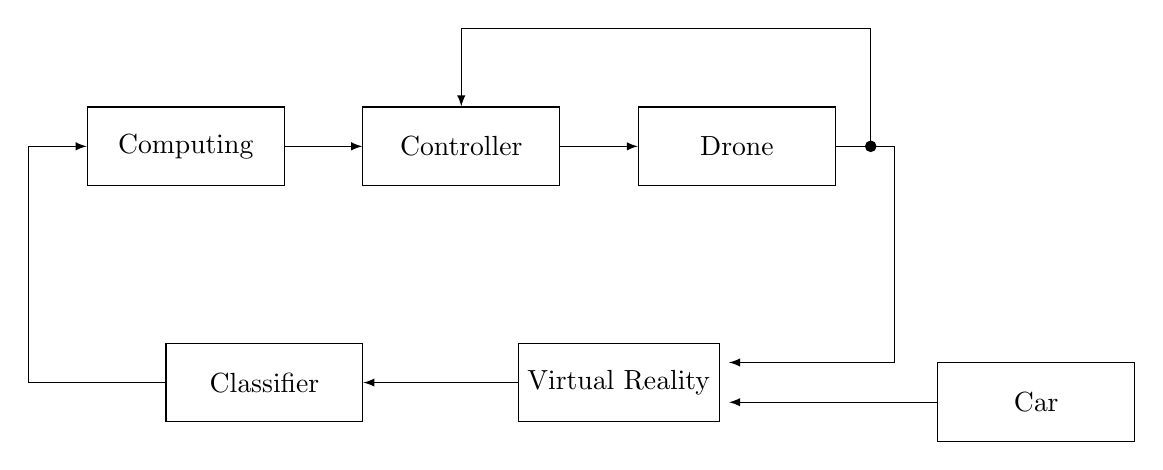
\begin{tikzpicture}[node distance=2cm]
			
			%Blocks
			\node (virtualReality) at (2.5,0) [rectangle, draw, text centered, minimum width=2.5cm, 
			minimum height=1cm] {Virtual Reality};
			\node (classifier) at (-2,0) [rectangle, draw, text centered, minimum width=2.5cm, 
			minimum height=1cm] {Classifier};
			\node (computing) at (-3,3)  [rectangle, draw, text centered, minimum width=2.5cm, 
			minimum height=1cm] {Computing};
			\node (controller) at (0.5,3) [rectangle, draw, text centered, minimum 
			width=2.5cm,minimum height=1cm] {Controller};
			\node (car) at (7.8,-0.25) [rectangle, draw, text centered, minimum width=2.5cm, 
			minimum height=1cm] {Car};
			\node (drone) at (4.0,3) [rectangle, draw, text centered, minimum width=2.5cm, minimum 
			height=1cm] {Drone};
			
			%Links
			\draw [-latex] (virtualReality.west) -- (classifier.east);
			\draw [-latex] (classifier.west) -- (-5.0,0) -- (-5.0,3) -- (computing.west);
			\draw [-latex] (computing.east) -- (controller.west);
			\draw [-latex] (controller.east) -- (drone.west);
			\draw [-latex] (car.west) -- (3.9,-0.25);
			\draw [-latex] (drone.east) -- (6.0,3) -- (6.0,0.255) -- (3.9,0.255);
			\draw [-latex] (5.7,3) -- (5.7,4.5) -- (0.5,4.5) -- (controller.north);
			\node (circle) at (5.7,3) [circle, draw, scale=0.4, fill=black] {};
			
			\end{tikzpicture}
	\end{center}

\end{figure}

\newpage

%%%%%%%%%%%%%%%%%%%%%%%%%%%%%%%%%%%%%%%%%%%%%%%%%%%%%%%%%%%%%%%%%%%%%%%%%%%%%%%%%%%%%%%%%%%%%%%%%%%%

\section{Example \theblockDiagram}
\stepcounter{blockDiagram}

\begin{figure}[h]
	\begin{center}
		\begin{tikzpicture}
		
		%Reference system
		\draw[dashed] (0,0) coordinate -- (0,1) coordinate;
		\draw[-latex] (0,1) coordinate -- (0,3) coordinate node[above left]{$y$};
		\draw[dashed] (0,0) coordinate -- (1,0) coordinate;
		\draw[-] (1,0) coordinate -- (3,0) coordinate node[above right]{$-x$};
		\draw[dashed] (0,0) coordinate -- (-1.2,0) coordinate;
		\draw[-latex] (-1.2,0) coordinate -- (-3,0) coordinate node[above left]{$x$};
		\node (circle) at (0,0) [circle, draw, dashed, minimum size=0.5cm]{};
		\node[circle,draw,black,scale=0.3, fill=black] at (0,0) {};
		\draw (0,-0.25) coordinate node[below left]{$z$};
		
		%Camera
		\draw[-, line width=1.25pt] (1,1) coordinate -- (-1,1) coordinate;
		\draw[-, line width=1.25pt] (1,-1) coordinate -- (-1,-1) coordinate;
		\draw[-, line width=1.25pt] (1,-1) coordinate -- (1,1) coordinate;
		\draw[-, line width=1.25pt] (-1,-1) coordinate -- (-1,1) coordinate;
		
		\draw[-, line width=1.25pt] (-1,-1) coordinate -- (-1.2,-1.2) coordinate;
		\draw[-, line width=1.25pt] (-1,1) coordinate -- (-1.2,1.2) coordinate;
		\draw[-, line width=1.25pt] (-1.2,1.2) coordinate -- (-1.2,-1.2) coordinate;
		
		\end{tikzpicture}
	\end{center}
	
\end{figure}

%%%%%%%%%%%%%%%%%%%%%%%%%%%%%%%%%%%%%%%%%%%%%%%%%%%%%%%%%%%%%%%%%%%%%%%%%%%%%%%%%%%%%%%%%%%%%%%%%%%%

\section{Example \theblockDiagram}
\stepcounter{blockDiagram}

\begin{figure}[h]
	\begin{center}
		\scalebox{0.8}{
			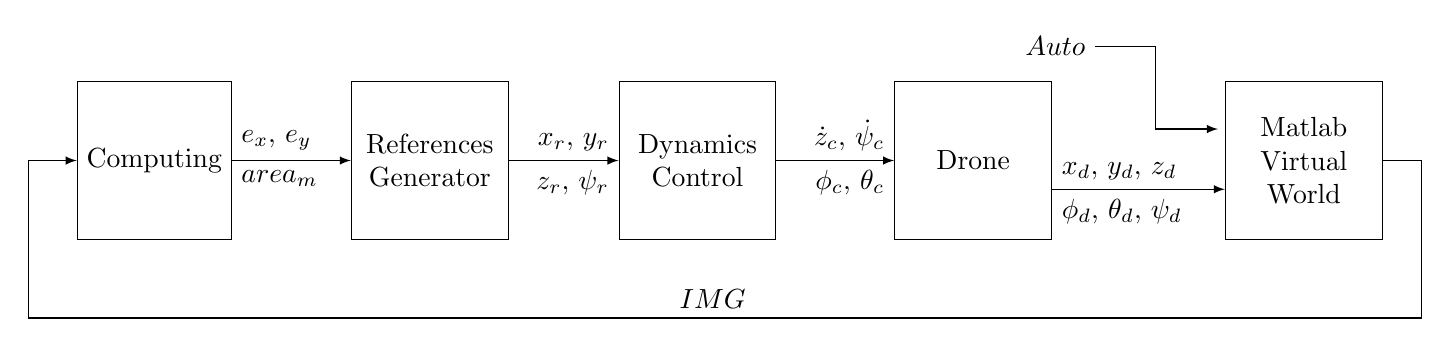
\begin{tikzpicture}
			
			%Computing block
			\node (computing) at (-4.2,0) [draw, rectangle, text centered, minimum width=1cm, 
			minimum height=2cm]{Computing};
			
			%Reference generator
			\node (referenceGenerator) at (-0.7,0) [draw, rectangle, minimum width=1cm, text 
			width=5em, minimum height=2cm, text centered]{References\\ Generator};
			
			%Trajectory controller
			\node (trajectoryController) at (2.7,0) [draw, rectangle, minimum width=1cm, minimum 
			height=2cm, text centered, text width=5em]{Dynamics\\ Control};
			
			%Drone
			\node (drone) at (6.2,0) [draw, rectangle, minimum width=1cm, minimum height=2cm, text 
			centered, text width=5em]{Drone};
			
			%Matlab virtual world
			\node (virtualWorld) at (10.4,0) [draw, rectangle, minimum width=1cm, minimum 
			height=2cm, text centered, text width=5em]{Matlab \\Virtual World};
			
			%Links among blocks
			\draw[-latex] (computing.east) node[above right]{$e_x,\,e_y$} node[below 
			right]{$area_m$}-- (referenceGenerator.west);
			\draw[-latex] (referenceGenerator.east) -- (trajectoryController.west) node[below 
			left]{$z_r,\,\psi_r$} node[above left]{$x_r,\,y_r$};
			\draw[-latex] (trajectoryController.east) -- (drone.west) node[above 
			left]{$\dot{z}_c,\,\dot{\psi}_c$} node[below left]{$\phi_c,\,\theta_c$};
			\draw[-latex] (drone.-20) node[below right]{$\phi_d,\,\theta_d,\,\psi_d$} node[above 
			right]{$x_d,\,y_d,\,z_d$} -- (virtualWorld.200);
			\draw[-latex] (virtualWorld.east) -- (11.9,0) coordinate -- (11.9,-2.0) coordinate 
			--(-5.8,-2.0) coordinate -- (-5.8,0) coordinate -- (computing.west);
			\draw (2.35,-2.0) coordinate node[above right]{$IMG$};
			
			%Link for connecting the car block
			\draw[-latex] (7.75,1.45) coordinate node[left]{$Auto$}-- (8.52,1.45) coordinate -- 
			(8.52,0.4) coordinate -- (9.31,0.4) coordinate;
			
			\end{tikzpicture}
		}
	\end{center}
	
\end{figure}

%%%%%%%%%%%%%%%%%%%%%%%%%%%%%%%%%%%%%%%%%%%%%%%%%%%%%%%%%%%%%%%%%%%%%%%%%%%%%%%%%%%%%%%%%%%%%%%%%%%%

\section{Example \theblockDiagram}
\stepcounter{blockDiagram}

\begin{figure}[h]
	\begin{center}
		\scalebox{0.7}{
			\begin{tikzpicture}
			
			%Initial links
			\draw[-latex] (-5.5,1.5) coordinate node[left]{$U_1$} -- (-4.5,1.5) coordinate;
			\draw[-latex] (-5.5,0.7) coordinate node[left]{$U_2$} -- (-4.5,0.7) coordinate;
			\draw[-latex] (-5.5,-0.7) coordinate node[left]{$U_3$} -- (-4.5,-0.7) coordinate;
			\draw[-latex] (-5.5,-1.5) coordinate node[left]{$U_3$} -- (-4.5,-1.5) coordinate;
			
			%Omega qr calculator block
			\node (omegaQRCalculator) at (-3.5,0) [draw, rectangle, minimum height=5cm, minimum 
			width=2cm, text centered, label={[align=center]below:Omega qr\\computation}]{};
			
			%Variables - omega qr calculator
			\draw (-3.8, 1.5) coordinate node[left]{$U_{1}$};
			\draw (-3.8, 0.7) coordinate node[left]{$U_{2}$};
			\draw (-3.8, -0.7) coordinate node[left]{$U_{3}$};
			\draw (-3.8, -1.5) coordinate node[left]{$U_{4}$};
			
			\draw (-2.5, 2.0) coordinate node[left]{$\Omega$};
			\draw (-2.5, 1.0) coordinate node[left]{$U_{1_{2}}$};
			\draw (-2.5, 0.0) coordinate node[left]{$U_{2_{2}}$};
			\draw (-2.5, -1.0) coordinate node[left]{$U_{3_{2}}$};
			\draw (-2.5, -2.0) coordinate node[left]{$U_{4_{2}}$};
			
			%Links between the omega and angles blocks
			\draw[-latex] (-2.5,2.0) coordinate -- (-1.75,2.0) coordinate -- (-1.75,-3.0) 
			coordinate -- (-1,-3.0) coordinate;
			\draw[-latex] (-2.5,1.0) coordinate -- (-1.95,1.0) coordinate -- (-1.95,4.0) coordinate 
			-- (6.5,4.0) coordinate -- (6.5,-1.5) coordinate -- (7,-1.5) coordinate;
			\draw[-latex] (-2.5,0.0) coordinate -- (-1,0.0) coordinate;
			\draw[-latex] (-2.5,-1.0) coordinate -- (-1,-1.0) coordinate;
			\draw[-latex] (-2.5,-2.0) coordinate -- (-1,-2.0) coordinate;
			
			%Angles block
			\node (anglesBlock) at (0,0) [draw, rectangle, minimum height=7cm, minimum width=2cm, 
			text centered, label={[align=center]below:Angles}]{};
			
			%Variables - angles
			\draw (-0.5,3.0) coordinate node[left]{$\dot{\phi}$};
			\draw (-0.5,2.0) coordinate node[left]{$\dot{\theta}$};
			\draw (-0.5,1.0) coordinate node[left]{$\dot{\psi}$};
			\draw (-0.3,0.0) coordinate node[left]{$U_2$};
			\draw (-0.3,-1.0) coordinate node[left]{$U_3$};
			\draw (-0.3,-2.0) coordinate node[left]{$U_4$};
			\draw (-0.4,-3.0) coordinate node[left]{$\Omega$};
			
			\draw (1.0, 2.5) coordinate node[left]{$\ddot{\phi}$};
			\draw (1.0, 0.0) coordinate node[left]{$\ddot{\theta}$};
			\draw (1.0, -2.5) coordinate node[left]{$\ddot{\psi}$};
			
			%First integrator block - angles
			\node (integrator1) at (3,0) [draw, rectangle, minimum height=1cm, minimum width=1cm, 
			text centered, label={[align=center]below:$\dot{\theta}$}]{$\cfrac{1}{s}$};
			\node (integrator2) at (3,2) [draw, rectangle, minimum height=1cm, minimum width=1cm, 
			text centered, label={[align=center]below:$\dot{\phi}$}]{$\cfrac{1}{s}$};
			\node (integrator3) at (3,-2) [draw, rectangle, minimum height=1cm, minimum width=1cm, 
			text centered, label={[align=center]below:$\dot{\psi}$}]{$\cfrac{1}{s}$};
			
			%Links between the angles and integrator blocks
			\draw[-latex] (1.0,2.5) coordinate -- (1.5,2.5) coordinate -- (1.5,2.0) coordinate -- 
			(integrator2.west);
			\draw[-latex] (1.0,0.0) coordinate -- (integrator1.west);
			\draw[-latex] (1.0,-2.5) coordinate -- (1.5,-2.5) coordinate -- (1.5,-2.0) coordinate 
			-- (integrator3.west);
			
			%Second integrators block - angles
			\node (integrator4) at (5,0) [draw, rectangle, minimum height=1cm, minimum width=1cm, 
			text centered, label={[align=center]below:$\theta$}]{$\cfrac{1}{s}$};
			\node (integrator5) at (5,2) [draw, rectangle, minimum height=1cm, minimum width=1cm, 
			text centered, label={[align=center]below:$\phi$}]{$\cfrac{1}{s}$};
			\node (integrator6) at (5,-2) [draw, rectangle, minimum height=1cm, minimum width=1cm, 
			text centered, label={[align=center]below:$\psi$}]{$\cfrac{1}{s}$};
			
			%Circle on the connection links
			\node[circle,draw,black,scale=0.2, fill=black] (A) at (4,0){};
			\node[circle,draw,black,scale=0.2, fill=black] (A) at (4.2,-2){};
			\node[circle,draw,black,scale=0.2, fill=black] (A) at (3.8,2){};
			
			%Links among blocks
			\draw[-latex] (4,0) coordinate -- (4,4.2) coordinate -- (-1.55,4.2) coordinate -- 
			(-1.55,2.0) coordinate -- (-1.0,2.0);
			\draw[-latex] (4.2,-2) coordinate -- (4.2,3.8) coordinate -- (-1.35,3.8) coordinate -- 
			(-1.35,1.0) coordinate -- (-1.0,1.0);
			\draw[-latex] (3.8,2) coordinate -- (3.8,4.4) coordinate -- (-1.15,4.4) coordinate -- 
			(-1.15,3.0) coordinate -- (-1.0,3.0);
			
			%Links among integrators blocks
			\draw[-latex] (integrator1.east) -- (integrator4.west);
			\draw[-latex] (integrator2.east) -- (integrator5.west);
			\draw[-latex] (integrator3.east) -- (integrator6.west);
			
			%Connection links between the integrators and displacement blocks
			\draw[-latex] (integrator5.east) -- (6.3,2) coordinate -- (6.3,1.5) coordinate -- 
			(7.0,1.5) coordinate;
			\draw[-latex] (integrator4.east) -- (6.7,0.0) coordinate -- (6.7,0.5) coordinate -- 
			(7.0,0.5) coordinate;
			\draw[-latex] (integrator6.east) -- (6.1,-2) coordinate -- (6.1,-0.5) coordinate -- 
			(7.0,-0.5) coordinate;
			
			%Displacement block
			\node (bloccoDisplacement) at (8,0) [draw, rectangle, minimum height=4cm, minimum 
			width=2cm, text centered, label={[align=center]below:Displacements}]{};
			
			%Variables - displacement
			\draw (7.5,1.5) coordinate node[left]{$\phi$};
			\draw (7.5,0.5) coordinate node[left]{$\theta$};
			\draw (7.5,-0.5) coordinate node[left]{$\psi$};
			\draw (7.65,-1.5) coordinate node[left]{$U_1$};
			
			\draw (8.9,1.25) coordinate node[left]{$\ddot{x}$};
			\draw (8.9,0.0) coordinate node[left]{$\ddot{y}$};
			\draw (8.9,-1.25) coordinate node[left]{$\ddot{z}$};
			
			%First integrators block - displacement
			\node (integrator7) at (11,0) [draw, rectangle, minimum height=1cm, minimum width=1cm, 
			text centered, label={[align=center]below:$\dot{y}$}]{$\cfrac{1}{s}$};
			\node (integrator8) at (11,2) [draw, rectangle, minimum height=1cm, minimum width=1cm, 
			text centered, label={[align=center]below:$\dot{x}$}]{$\cfrac{1}{s}$};
			\node (integrator9) at (11,-2) [draw, rectangle, minimum height=1cm, minimum width=1cm, 
			text centered, label={[align=center]below:$\dot{z}$}]{$\cfrac{1}{s}$};
			
			%Links for the displacement block
			\draw[-latex] (9,1.25) coordinate -- (10.1,1.25) coordinate -- (10.1,2) coordinate -- 
			(integrator8.west);
			\draw[-latex] (9,0.0) coordinate -- (integrator7.west);
			\draw[-latex] (9,-1.25) coordinate -- (10.1,-1.25) coordinate -- (10.1,-2) coordinate 
			-- (integrator9.west);
			
			%Second block of integrators - displacement
			\node (integrator10) at (13,0) [draw, rectangle, minimum height=1cm, minimum width=1cm, 
			text centered,label={[align=center]below:$y$}]{$\cfrac{1}{s}$};
			\node (integrator11) at (13,2) [draw, rectangle, minimum height=1cm, minimum width=1cm, 
			text centered,label={[align=center]below:$x$}]{$\cfrac{1}{s}$};
			\node (integrator12) at (13,-2) [draw, rectangle, minimum height=1cm, minimum 
			width=1cm, text centered,label={[align=center]below:$z$}]{$\cfrac{1}{s}$};
			
			%Connections between the two integrators blocks
			\draw[-latex] (integrator7.east) -- (integrator10.west);
			\draw[-latex] (integrator8.east) -- (integrator11.west);
			\draw[-latex] (integrator9.east) -- (integrator12.west);
			
			%Final interconnections
			\draw[-latex] (integrator10.east) -- (15,0) coordinate node[right]{$y$};
			\draw[-latex] (integrator11.east) -- (15,2) coordinate node[right]{$x$};
			\draw[-latex] (integrator12.east) -- (15,-2) coordinate node[right]{$z$};
			
			\end{tikzpicture}
		}
	\end{center}
	
\end{figure}

%%%%%%%%%%%%%%%%%%%%%%%%%%%%%%%%%%%%%%%%%%%%%%%%%%%%%%%%%%%%%%%%%%%%%%%%%%%%%%%%%%%%%%%%%%%%%%%%%%%%

\section{Example \theblockDiagram}
\stepcounter{blockDiagram}

\begin{figure}[h]
	\begin{center}
		\scalebox{0.85}{
			
			\begin{tikzpicture}
			\node (feedbackController) at (0,1.25) [draw, ellipse, text centered, minimum 
			height=1cm, fill=yellow!25, text width=10em]{\textbf{ROS NODE}\\Feedback Controller in 
			Simulink};
			\node (robotSimulator) at (0,-4.25) [draw, ellipse, text centered, minimum 
			height=2cm,fill=yellow!25, text width=10em]{\textbf{ROS NODE}\\Robot Simulator};
			
			\node (odom) at (-4,-1.5) [draw, rectangle, text centered, text width=19em, minimum 
			height=2cm, rounded corners=5pt]{\textbf{Topic}: /odom\\\textbf{Message type}: 
			nav\_msgs/Odometry};
			\node (mobileBase) at (4,-1.5) [draw, rectangle, text centered, text width=19em, 
			minimum height=2cm, rounded corners=5pt]{\textbf{Topic}: 
			/mobile\_base/commands/velocity\\\textbf{Message type}: geometry\_msgs/Twist};
			
			\draw[-latex, line width=1.25pt] (feedbackController) [out=0, in=90] to (mobileBase);
			\draw[-latex, line width=1.25pt] (mobileBase) [out=270, in=0] to (robotSimulator);
			\draw[-latex, line width=1.25pt] (robotSimulator) [out=180, in=270] to (odom);
			\draw[-latex, line width=1.25pt] (odom) [out=90, in=180] to (feedbackController); 
			
			\end{tikzpicture}
		}
	\end{center}
\end{figure}

%%%%%%%%%%%%%%%%%%%%%%%%%%%%%%%%%%%%%%%%%%%%%%%%%%%%%%%%%%%%%%%%%%%%%%%%%%%%%%%%%%%%%%%%%%%%%%%%%%%%

\section{Example \theblockDiagram}
\stepcounter{blockDiagram}

\begin{figure}[h]
	\begin{center}
		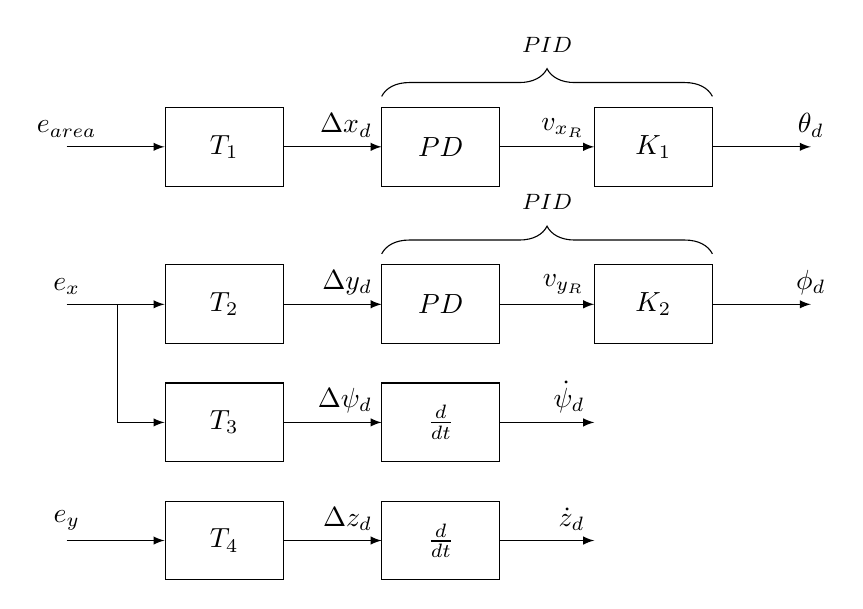
\begin{tikzpicture}
		
		%Nodes in the first part of the scheme
		\node (firstTransformation) at (-2,0.5) [draw, rectangle, minimum width=1.5cm, minimum 
		height=1cm, text centered]{$T_1$};
		
		\node (firstPD) at (0.75,0.5) [draw, text centered, minimum width=1.5cm, minimum 
		height=1cm]{$PD$};
		
		\node (firstK) at (3.45,0.5) [draw, text centered, minimum width=1.5cm, minimum 
		height=1cm]{$K_1$};
		
		\draw [decorate,decoration={brace, mirror, amplitude=10pt,raise=4pt},yshift=0pt]
		(4.2,1) -- (0,1) node [black,midway,yshift=0.8cm] {\footnotesize $PID$};
		
		%Links
		\draw[-latex] (-4,0.5) coordinate node[above]{$e_{area}$} -- (firstTransformation.west);
		
		\draw[-latex] (firstTransformation.east) -- (0,0.5) coordinate node[above left]{$\Delta 
		x_d$};
		
		\draw[-latex] (firstPD.east) -- (2.7,0.5) coordinate node[above left]{$v_{{x}_R}$};
		
		\draw[-latex] (firstK.east) -- (5.45,0.5) coordinate node[above]{$\theta_d$};
		
		
		%Nodes in the second part of the scheme
		\node (secondTransformation) at (-2,-1.5) [draw, rectangle, minimum width=1.5cm, minimum 
		height=1cm, text centered]{$T_2$};
		
		\node (secondPD) at (0.75,-1.5) [draw, text centered, minimum width=1.5cm, minimum 
		height=1cm]{$PD$};
		
		\node (secondK) at (3.45,-1.5) [draw, text centered, minimum width=1.5cm, minimum 
		height=1cm]{$K_2$};
		
		\draw [decorate,decoration={brace, mirror, amplitude=10pt,raise=4pt},yshift=0pt]
		(4.2,-1.0) -- (0,-1.0) node [black,midway,yshift=0.8cm] {\footnotesize
			$PID$};
		
		%Links among blocks
		\draw[-latex] (-4,-1.5) coordinate node[above]{$e_x$} -- (secondTransformation.west);
		
		\draw[-latex] (secondTransformation.east) -- (0,-1.5) coordinate node[above left]{$\Delta 
		y_d$};
		
		\draw[-latex] (secondPD.east) -- (2.7,-1.5) coordinate node[above left]{$v_{{y}_R}$};
		
		\draw[-latex] (secondK.east) -- (5.45,-1.5) coordinate node[above]{$\phi_d$};
		
		
		%Nodes in the third part of the scheme
		\node (thirdTransformation) at (-2,-3.0) [draw, rectangle, minimum width=1.5cm, minimum 
		height=1cm, text centered]{$T_3$};
		
		\node (thirdPD) at (0.75,-3.0) [draw, text centered, minimum width=1.5cm, minimum 
		height=1cm]{$\frac{d}{dt}$};
		
		%Links among blocks
		\draw[-latex] (-3.35, -1.5) coordinate --  (-3.35,-3.0) coordinate -- 
		(thirdTransformation.west);
		
		\draw[-latex] (thirdTransformation.east) -- (0,-3.0) coordinate node[above left]{$\Delta 
		\psi_d$};
		
		\draw[-latex] (thirdPD.east) -- (2.7,-3.0) coordinate node[above left]{$\dot{\psi}_d$};
		
		
		%Nodes of the fourth part of the scheme
		\node (fourthTransformation) at (-2,-4.5) [draw, rectangle, minimum width=1.5cm, minimum 
		height=1cm, text centered]{$T_4$};
		
		\node (fourthPD) at (0.75,-4.5) [draw, text centered, minimum width=1.5cm, minimum 
		height=1cm]{$\frac{d}{dt}$};
		
		%Links among blocks
		\draw[-latex] (-4,-4.5) coordinate node[above]{$e_y$} -- (fourthTransformation.west);
		
		\draw[-latex] (fourthTransformation.east) -- (0,-4.5) coordinate node[above left]{$\Delta 
		z_d$};
		
		\draw[-latex] (fourthPD.east) -- (2.7,-4.5) coordinate node[above left]{$\dot{z}_d$};
		
		
		\end{tikzpicture}
	\end{center}
	
\end{figure}

\newpage

%%%%%%%%%%%%%%%%%%%%%%%%%%%%%%%%%%%%%%%%%%%%%%%%%%%%%%%%%%%%%%%%%%%%%%%%%%%%%%%%%%%%%%%%%%%%%%%%%%%%

\section{Example \theblockDiagram}
\stepcounter{blockDiagram}

\begin{figure}[h]
	\begin{center}
		\scalebox{1}{
			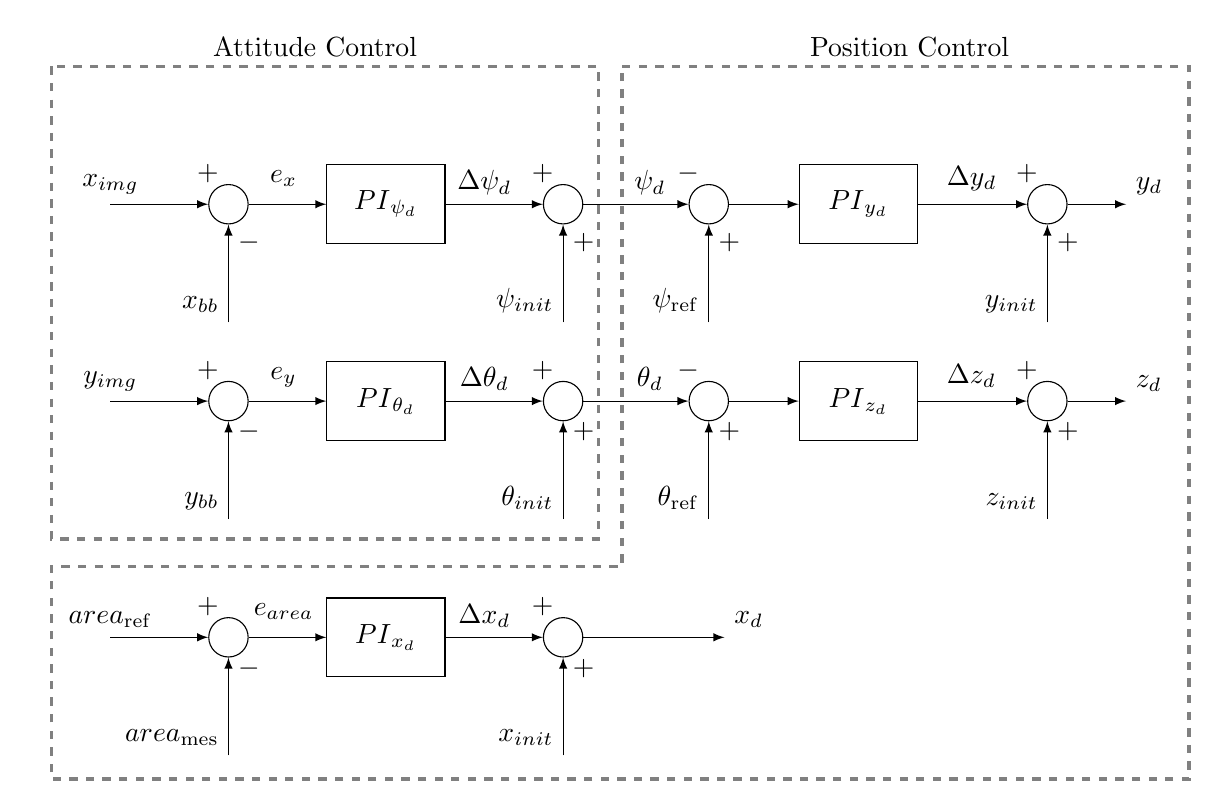
\begin{tikzpicture}
			
			%Attitude controller
			\node (attitudeController) at (-3.40,-1.25) [rectangle, label=Attitude Control, text 
			centered, minimum height=6cm, minimum width=7.3cm]{};
			
			\draw[dashed, gray, line width=1.25pt] (-6.75,1.75) coordinate -- (-6.75,-4.25) 
			coordinate -- (0.2,-4.25) coordinate -- (0.2,1.75) coordinate -- (-6.75,1.75) 
			coordinate;
			
			%Position controller
			\draw[dashed, gray, line width=1.25pt] (0.5, 1.75) coordinate -- (7.7, 1.75) coordinate 
			-- (7.7, -7.3) coordinate --  (-6.75,-7.3) coordinate -- (-6.75,-4.6) coordinate --  
			(0.5,-4.6) coordinate -- (0.5,1.75) coordinate;
			
			\node (positionController) at (4.15,-1.25) [label=Position Control, text centered, 
			minimum width=2.65cm, minimum height=6cm, rectangle]{};
			
			%Blocks in the first part of the scheme
			\node (adder1) at (-4.5,0) [draw, circle, text centered, minimum size=0.5cm]{};
			
			\node (pi1) at (-2.5,0) [draw, rectangle, text centered, minimum height=1.0cm, minimum 
			width=1.5cm]{$\text{PI}_{\psi_d}$};
			
			\node (adder2) at (-0.25,0) [draw, circle, text centered, minimum size=0.5cm]{};
			
			\node (adder20) at (1.6,0) [draw, circle, text centered, minimum size=0.5cm]{};
			
			\node (pi2) at (3.5,0) [draw, rectangle, text centered, minimum height=1cm, minimum 
			width=1.5cm]{$\text{PI}_{y_d}$};
			
			\node (adder6) at (5.9,0) [draw, circle, text centered, minimum size=0.5cm]{};
			
			%Links among blocks
			\draw[-latex] (-6.0,0) coordinate node[above]{$x_{img}$} -- (adder1.west);
			\draw[-latex] (-4.5,-1.5) coordinate node[above left]{$x_{bb}$} -- (adder1.south);
			
			\draw[-latex] (adder1.east) -- (pi1.west);
			\draw[-latex] (pi1.east) -- (adder2.west);
			
			\draw[-latex] (-0.25,-1.5) coordinate node[above left]{$\psi_{init}$}-- (adder2.south);
			
			\draw[-latex] (1.6,-1.5) coordinate node[above left]{$\psi_\mathrm{ref}$} -- 
			(adder20.south);
			
			\draw[-latex] (adder2.east) -- (adder20.west);
			\draw[-latex] (adder20.east) -- (pi2.west);
			\draw[-latex] (pi2.east) -- (adder6.west);
			\draw (4.5,0.05) node[above right]{$\Delta y_d$};
			
			\draw[-latex] (5.9,-1.5) coordinate node[above left]{$y_{init}$} -- (adder6.south);
			\draw[-latex] (adder6.east) -- (6.9,0) coordinate node[above right]{$y_d$};
			
			%Signs
			\draw (-4.5,0.15) coordinate node[above left]{$+$};
			\draw (-4.5,-0.25) coordinate node[below right]{$-$};
			
			\draw (-0.25,0.15) coordinate node[above left]{$+$};
			\draw (-0.25,-0.25) coordinate node[below right]{$+$};
			
			\draw (1.6,0.15) coordinate node[above left]{$-$};
			\draw (1.6,-0.25) coordinate node[below right]{$+$};
			
			\draw (5.9,0.15) coordinate node[above left]{$+$};
			\draw (5.9,-0.25) coordinate node[below right]{$+$};
			
			%Errors
			\draw (-3.8,0.55) coordinate node[below]{$e_x$};
			\draw (-1.25,0.55) coordinate node[below]{$\Delta \psi_d$};
			\draw (0.85,0.55) coordinate node[below]{$\psi_d$};
			
			
			%Blocks in the second part of the scheme
			\node (adder3) at (-4.5,-2.5) [draw, circle, text centered, minimum size=0.5cm]{};
			
			\node (pi3) at (-2.5,-2.5) [draw, rectangle, text centered, minimum height=1.0cm, 
			minimum width=1.5cm]{$\text{PI}_{\theta_d}$};
			
			\node (adder4) at (-0.25,-2.5) [draw, circle, text centered, minimum size=0.5cm]{};
			
			\node (adder50) at (1.6,-2.5) [draw, circle, text centered, minimum size=0.5cm]{};
			
			\node (pi4) at (3.5,-2.5) [draw, rectangle, text centered, minimum height=1cm, minimum 
			width=1.5cm]{$\text{PI}_{z_d}$};
			
			\node (adder7) at (5.9,-2.5) [draw, circle, text centered, minimum size=0.5cm]{}; 
			
			%Links among blocks
			\draw[-latex] (-6.0,-2.5) coordinate node[above]{$y_{img}$} -- (adder3.west);
			\draw[-latex] (-4.5,-4.0) coordinate node[above left]{$y_{bb}$} -- (adder3.south);
			
			\draw[-latex] (adder3.east) -- (pi3.west);
			\draw[-latex] (pi3.east) -- (adder4.west);
			
			\draw[-latex] (-0.25,-4.0) coordinate node[above left]{$\theta_{init}$} -- 
			(adder4.south);
			
			\draw[-latex] (1.6,-4.0) coordinate node[above left]{$\theta_\mathrm{ref}$} -- 
			(adder50.south);
			
			\draw[-latex] (adder4.east) -- (adder50.west);
			\draw[-latex] (adder50.east) -- (pi4.west);
			\draw[-latex] (pi4.east) -- (adder7.west); 
			\draw (4.5,-2.45) coordinate node[above right]{$\Delta z_d$};
			
			\draw[-latex] (5.9,-4.0) node[above left]{$z_{init}$} -- (adder7.south);
			
			\draw[-latex] (adder7.east) -- (6.9,-2.5) coordinate node[above right]{$z_d$};
			
			%Sings
			\draw (-4.5,-2.35) coordinate node[above left]{$+$};
			\draw (-4.5,-2.65) coordinate node[below right]{$-$};
			
			\draw (-0.25,-2.35) coordinate node[above left]{$+$};
			\draw (-0.25,-2.65) coordinate node[below right]{$+$};
			
			\draw (1.6,-2.35) coordinate node[above left]{$-$};
			\draw (1.6,-2.65) coordinate node[below right]{$+$};
			
			\draw (5.9,-2.35) coordinate node[above left]{$+$};
			\draw (5.9,-2.65) coordinate node[below right]{$+$};
			
			%Errors
			\draw (-3.8,-1.95) coordinate node[below]{$e_y$};
			\draw (-1.25,-1.95) coordinate node[below]{$\Delta \theta_d$};
			\draw (0.85,-1.95) coordinate node[below]{$\theta_d$};
			
			%Blocks in the third part of the scheme
			\node (adder5) at (-4.5,-5.5) [draw, circle, text centered, minimum size=0.5cm]{};
			
			\node (pi5) at (-2.5,-5.5) [draw, rectangle, text centered, minimum height=1.0cm, 
			minimum width=1.5cm]{$\text{PI}_{x_d}$};
			
			\node (adder8) at (-0.25,-5.5) [draw, circle, text centered, minimum size=0.5cm]{};
			
			%Links
			\draw[-latex] (-6.0,-5.5) coordinate node[above]{$area_{\mathrm{ref}}$} -- 
			(adder5.west);
			\draw[-latex] (-4.5,-7.0) coordinate node[above left]{$area_{\mathrm{mes}}$} -- 
			(adder5.south);
			
			\draw[-latex] (adder5.east) -- (pi5.west);
			
			\draw[-latex] (pi5.east) -- (adder8.west);
			\draw (-1.25,-5.5) coordinate node[above]{$\Delta x_d$};
			
			\draw[-latex] (-0.25,-7.0) coordinate node[above left]{$x_{init}$} -- (adder8.south);
			
			%Signs
			\draw (-4.5,-5.35) coordinate node[above left]{$+$};
			\draw (-4.5,-5.65) coordinate node[below right]{$-$};
			
			\draw (-0.25,-5.35) coordinate node[above left]{$+$};
			\draw (-0.25,-5.65) coordinate node[below right]{$+$};
			
			\draw[-latex] (adder8.east) -- (1.8,-5.5) coordinate node[above right]{$x_d$};
			
			%Errors
			\draw (-3.8,-4.95) coordinate node[below]{$e_{area}$};
			
			
			\end{tikzpicture}
		}
	\end{center}

\end{figure}

%%%%%%%%%%%%%%%%%%%%%%%%%%%%%%%%%%%%%%%%%%%%%%%%%%%%%%%%%%%%%%%%%%%%%%%%%%%%%%%%%%%%%%%%%%%%%%%%%%%%

\section{Example \theblockDiagram}
\stepcounter{blockDiagram}

\begin{figure}[h]
	\begin{center}
		\scalebox{1}{
			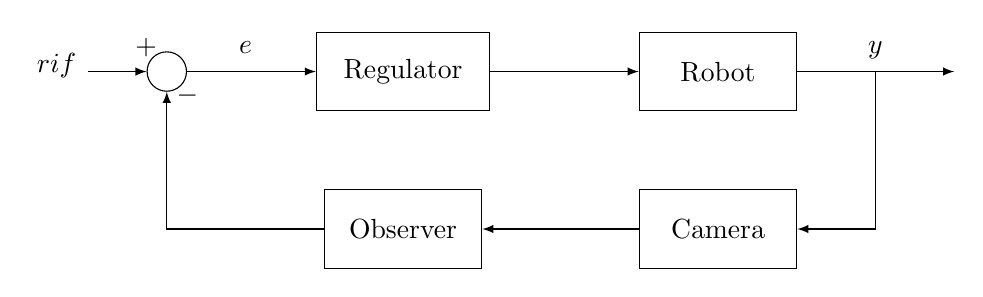
\begin{tikzpicture}[node distance=2cm]
			
			%Nodes
			\node (adder) at (0,0) [draw, circle, text centered, minimum size=0.5cm]{};
			
			\node (regulator) at (3,0) [draw, rectangle, text centered, minimum width=2.2cm, 
			minimum height=1cm]{Regulator};
			
			\node (robot) at (7,0) [draw, rectangle, text centered, minimum width=2cm, minimum 
			height=1cm]{Robot};
			
			\node (camera) at (7,-2) [draw, rectangle, text centered, minimum width=2cm, minimum 
			height=1cm]{Camera};
			
			\node (observer) at (3,-2) [draw, rectangle, text centered, minimum width=2cm, minimum 
			height=1cm]{Observer};
			
			%Links
			\draw[-latex] (adder) --  (regulator);
			\draw[-latex] (camera) -- (observer);
			\draw[-latex] (regulator) -- (robot);
			\draw[-latex] (observer.west) -- (0,-2) coordinate -- (adder.south);
			\draw[-latex] (robot.east) -- (10,0) coordinate;
			\draw[-latex] (9,0) coordinate -- (9,-2) coordinate -- (camera.east);
			\draw[-latex] (-1,0) coordinate -- (adder.west);
			
			%Variables
			\draw (9, 0.5) coordinate node[below]{$y$};
			\draw (1, 0.5) coordinate node[below]{$e$};
			\draw (-1.4,0.35) coordinate node[below]{$rif$};
			\draw (0,0.55) coordinate node[below left]{$+$};
			\draw (0,-0.55) coordinate node[above right]{$-$};
			
			\end{tikzpicture}
		}
	\end{center}
\end{figure}

\newpage

%%%%%%%%%%%%%%%%%%%%%%%%%%%%%%%%%%%%%%%%%%%%%%%%%%%%%%%%%%%%%%%%%%%%%%%%%%%%%%%%%%%%%%%%%%%%%%%%%%%%

\section{Example \theblockDiagram}
\stepcounter{blockDiagram}

\begin{figure}[h]
	\begin{center}
		\scalebox{0.72}{
			\begin{tikzpicture}
			
			%Yaw angle
			\node (yawAngle) at (0,0) [draw, rectangle, minimum height=2cm, minimum width=2cm, text 
			centered]{};
			\draw (1,1) coordinate -- (1.2,1.2) coordinate;
			\draw (1,-1) coordinate -- (1.2,-1.2) coordinate;
			\draw (1.2,-1.2) coordinate -- (1.2,1.2) coordinate;
			
			%Drawing the angle
			\draw (1.8,0) coordinate -- (2.2,0) coordinate;
			\draw[-latex, line width=1.0pt] (2.0,0) coordinate -- (2.0, -1) coordinate node[above 
			right]{$\psi_d$};
			
			%Reference system
			\draw[-latex] (-4,2) coordinate -- (-4,-1) coordinate node[above left]{$z$};
			\draw[-latex] (-4,2) coordinate -- (-2,2) coordinate node[above]{$x$};
			\node (circle) at (-4,2) [circle, draw, minimum size=0.5cm]{};
			\node[circle,draw,black,scale=0.2, fill=black] (A) at (-4,2) {};
			\draw (-4.25,2) coordinate node[above left]{$y$};
			
			%Dividing line among schems
			\draw[dashed, draw=gray] (-6,-2) coordinate -- (6,-2) coordinate;
			
			%Roll angle
			\node (rollAngle) at (0,-5) [draw, rectangle, minimum height=2cm, minimum width=2cm, 
			text centered]{};
			\draw (1,-4) coordinate -- (1.2,-3.8) coordinate;
			\draw (1,-6) coordinate -- (1.2,-6.2) coordinate;
			\draw (1.2,-3.8) coordinate -- (1.2,-6.2) coordinate;
			
			%Roll angle drawing
			\draw (1.8,-5) coordinate -- (2.2,-5) coordinate;
			\draw[-latex, line width=1.0pt] (2.0,-5) coordinate -- (2.0, -6) coordinate node[above 
			right]{$\phi_d$};
			
			%Reference system
			\draw[-latex] (-4,-3) coordinate -- (-2,-3) coordinate node[above]{$x$};
			\draw[-latex] (-4,-3) coordinate -- (-4,-6) coordinate node[above left]{$z$};
			\node (circle) at (-4,-3) [circle, draw, minimum size=0.5cm]{};
			\node[circle,draw,black,scale=0.2, fill=black] (A) at (-4,-3) {};
			\draw (-4.25,-3) coordinate node[above left]{$y$};
			
			%Diving line among schemes
			\draw[dashed, draw=gray] (-6,-7) coordinate -- (6,-7) coordinate;
			
			%Pitch angle
			\node (rollAngle) at (0,-9) [draw, rectangle, minimum height=2cm, minimum width=2cm, 
			text centered]{};
			\draw (1,-8) coordinate -- (1.2,-7.8) coordinate;
			\draw (1,-10) coordinate -- (1.2,-10.2) coordinate;
			\draw (1.2,-7.8) coordinate -- (1.2,-10.2) coordinate;
			
			%Drawing the angle
			\draw (0,-10.8) coordinate -- (0,-11.2) coordinate;
			\draw[-latex, line width=1.0pt] (0,-11) coordinate -- (1.0, -11) coordinate node[above 
			right]{$\theta_d$};
			
			%Reference system
			\draw[-latex] (-4,-10.5) coordinate -- (-2,-10.5) coordinate node[above]{$x$};
			\draw[-latex] (-4,-10.5) coordinate -- (-4,-8) coordinate node[above left]{$y$};
			\node (circle) at (-4,-10.5) [circle, draw, minimum size=0.5cm]{};
			\node[circle,draw,black,scale=0.2, fill=black] (A) at (-4,-10.5) {};
			\draw (-4.25,-10.5) coordinate node[above left]{$z$};
			
			
			\end{tikzpicture}
		}
	\end{center}

\end{figure}

%%%%%%%%%%%%%%%%%%%%%%%%%%%%%%%%%%%%%%%%%%%%%%%%%%%%%%%%%%%%%%%%%%%%%%%%%%%%%%%%%%%%%%%%%%%%%%%%%%%%

\section{Example \theblockDiagram}
\stepcounter{blockDiagram}

\begin{figure}[h]
	\begin{center}
		\scalebox{0.95}{
		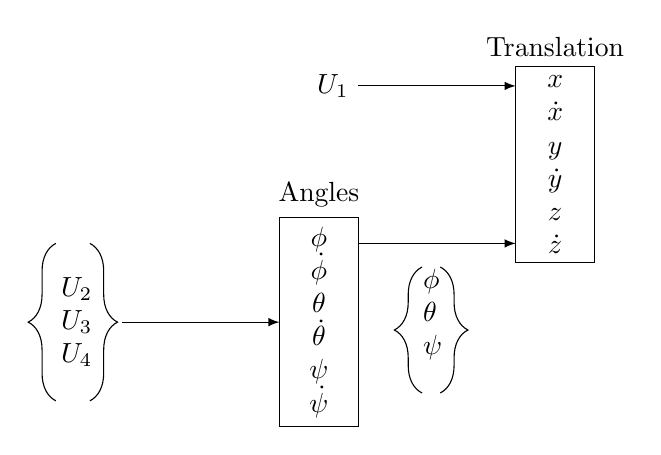
\begin{tikzpicture}
		
		%Drawing first rectangle
		\node (firstRectangle) at (0,0) [draw, rectangle, text centered, text width=1em, minimum 
		width=1cm, minimum height=2cm, label={Angles}]{$\phi$ \\ $\dot{\phi}$ \\ 
		$\theta$ \\ $\dot{\theta}$ \\ $\psi$ \\ $\dot{\psi}$};
		
		%Drawing second rectangle
		\node (secondRectangle) at (3,2) [draw, rectangle, text centered, text width=1em, minimum 
		width=1cm, minimum height=2cm, label={Translation}]{$x$ \\ $\dot{x}$ \\ $y$ \\ 
		$\dot{y}$ \\ $z$ \\ $\dot{z}$};
		
		%First arrow
		\draw[-latex] (0.5,1) coordinate -- (2.5,1) coordinate;
		\draw (1.5,0.8) coordinate node[below, text width=1em]{$\phi$ \\ $\theta$ \\ $\psi$};
		\draw [decorate,decoration={brace,amplitude=10pt,mirror,raise=4pt},yshift=0pt]
		(1.45,0.7) -- (1.45,-0.9) node [black,midway,xshift=0.8cm] {};
		\draw [decorate,decoration={brace,amplitude=10pt,raise=4pt},yshift=0pt]
		(1.40,0.7) -- (1.40,-0.9) node [black,midway,xshift=0.8cm] {};
		
		%Second arrow
		\draw[latex-] (-0.5,0) coordinate -- (-2.5,0) coordinate;
		\draw (-2.8,0) coordinate node[left, text width=1em]{$U_2$ \\ $U_3$ \\ $U_4$};
		\draw [decorate,decoration={brace,amplitude=10pt,mirror,raise=4pt},yshift=0pt]
		(-3.2,1) -- (-3.2,-1) node [black,midway,xshift=0.8cm] {};
		\draw [decorate,decoration={brace,amplitude=10pt,raise=4pt},yshift=0pt]
		(-3.05,1) -- (-3.05,-1) node [black,midway,xshift=0.8cm] {};
		
		%Third arrow
		\draw[-latex] (0.5,3) coordinate -- (2.5,3) coordinate;
		\draw (0.5,3) coordinate node[left]{$U_1$};
		
		\end{tikzpicture}
	}
	\end{center}

\end{figure}

\newpage

%%%%%%%%%%%%%%%%%%%%%%%%%%%%%%%%%%%%%%%%%%%%%%%%%%%%%%%%%%%%%%%%%%%%%%%%%%%%%%%%%%%%%%%%%%%%%%%%%%%%

\section{Example \theblockDiagram}
\stepcounter{blockDiagram}

\begin{figure}[h]
	\begin{center}
			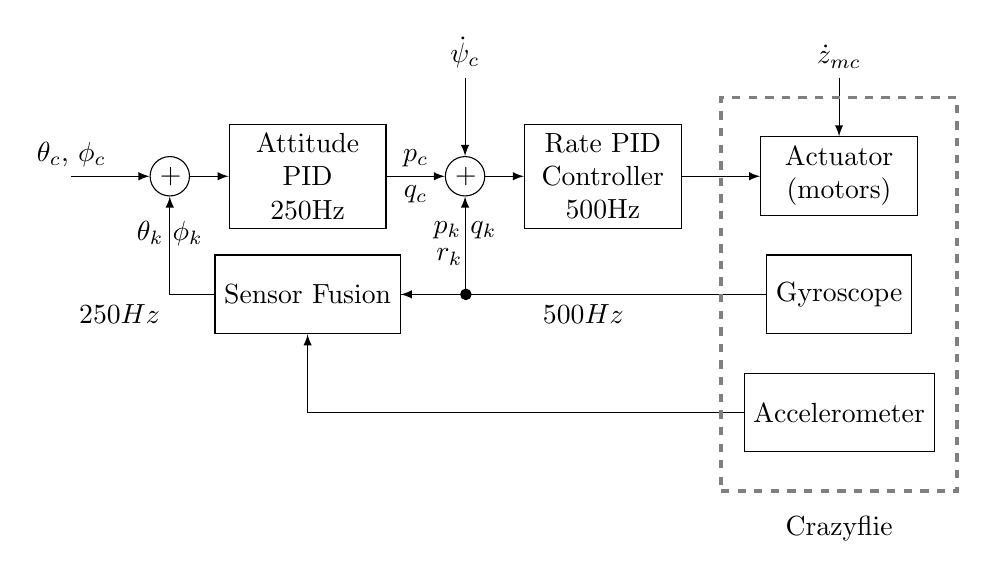
\begin{tikzpicture}
			
			%Blocks of the scheme
			\node (attitudePID) at (3.5,0) [draw, rectangle, minimum width=1cm, minimum height=1cm, 
			text centered, text width=5em]{Attitude PID\\250Hz};
			\node (ratePID) at (7.25,0) [draw, rectangle, minimum width=1cm, minimum height=1cm, 
			text centered, text width=5em]{Rate PID\\Controller\\500Hz};
			\node (actuators) at (10.25,0) [draw, rectangle, minimum width=1cm, minimum height=1cm, 
			text centered, text width=5em]{Actuator\\(motors)};
			\node (gyroscope) at (10.25,-1.5) [draw, rectangle, minimum width=1cm, minimum 
			height=1cm, text centered]{Gyroscope};
			\node (accelerometer) at (10.25,-3) [draw, rectangle, minimum width=1cm, minimum 
			height=1cm, text centered]{Accelerometer};
			\node (sensorFusion) at (3.5,-1.5) [draw, rectangle, minimum width=1cm, minimum 
			height=1cm, text centered]{Sensor Fusion};
			
			%Adders
			\node (adder1) at (1.75,0) [draw, circle, text centered, minimum size=0.5cm]{};
			\node (adder2) at (5.5,0) [draw, circle, text centered, minimum size=0.5cm]{};
			
			%Bubblies
			\node (coordinates1) at (5.51,-1.5) [circle, draw, scale=0.4, fill=black]{};
			
			%Linx
			\draw[-latex] (0.5,0) coordinate node[above]{$\theta_c$, $\phi_c$} -- (adder1);
			\draw[-latex] (adder1)   -- (attitudePID);
			\draw[-latex] (attitudePID) -- node[above]{$p_c$} node[below]{$q_c$} (adder2);
			\draw[-latex] (adder2) -- (ratePID);
			\draw[-latex] (ratePID) -- (actuators);
			\draw[-latex] (gyroscope) -- node[below]{$500Hz$} (sensorFusion);
			\draw[-latex] (accelerometer) -| (sensorFusion);
			\draw[-latex] (sensorFusion) -| (adder2);
			\draw[-latex] (sensorFusion) -| node[below left]{$250Hz$} (adder1);
			\draw[-latex] (5.5,1.25) coordinate node[above]{$\dot{\psi}_c$} -- (adder2);
			\draw[-latex] (10.25,1.25) coordinate node[above]{$\dot{z}_{mc}$} -- (actuators);
			
			%Senros fusion's outputs
			\draw (1.75,-0.45) coordinate node[below]{$\theta_k$ $\phi_k$};
			\draw (5.5,-0.45) coordinate node[below]{$p_k$ $q_k$};
			\draw (5.3,-0.8) coordinate node[below]{$r_k$};
			
			%Signs
			\draw (1.5,0) coordinate node[right]{$+$};
			\draw (5.25,0) coordinate node[right]{$+$};
			
			%Comments
			\node (Crazyflie) at (10.25,-1.5) [dashed, gray, rectangle, minimum width=3cm, 
			minimum height=5cm, draw, line width=1.25pt]{};
			\draw (10.25,-4.75) coordinate node[above]{Crazyflie};
			
			\end{tikzpicture}
	\end{center}
\end{figure}

%%%%%%%%%%%%%%%%%%%%%%%%%%%%%%%%%%%%%%%%%%%%%%%%%%%%%%%%%%%%%%%%%%%%%%%%%%%%%%%%%%%%%%%%%%%%%%%%%%%%

\section{Example \theblockDiagram}
\stepcounter{blockDiagram}

\begin{figure}[h]
	\begin{center}
			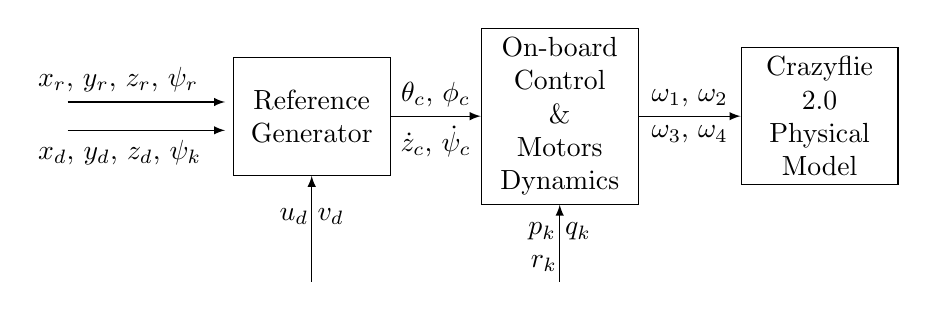
\begin{tikzpicture}
			
			%Blocks
			\node (ReferenceGenerator) at (-2.1,0) [draw, rectangle, minimum height=1.5cm, minimum 
			width=1cm, text centered, text width=5em]{Reference\\Generator};
			
			\node (OnboardCrazyflie) at (1.05,0) [draw, rectangle, minimum height=1.5cm, minimum 
			width=1cm, text centered, text width=5em]{On-board\\Control \\\& \\Motors Dynamics};
			
			\node (Crazyflie) at (4.35,0) [draw, rectangle, minimum height=1.5cm, minimum 
			width=1cm, text centered, text width=5em]{Crazyflie 2.0\\ Physical Model};
			
			%Links
			\draw[-latex] (ReferenceGenerator)  -- node[above]{$\theta_c$, $\phi_c$} 
			node[below]{$\dot{z}_c$, $\dot{\psi}_c$} (OnboardCrazyflie) ;
			\draw[-latex] (OnboardCrazyflie) -- node[above]{$\omega_1$, $\omega_2$} 
			node[below]{$\omega_3$, $\omega_4$}(Crazyflie);
			\draw[-latex] (-5.2,0.18)  -- (-3.2,0.18);
			\draw[-latex] (-5.2,-0.18) -- (-3.2,-0.18);
			\draw[-latex] (-2.1,-2.1) coordinate -- (ReferenceGenerator);
			\draw[-latex] (1.05,-2.1) coordinate -- (OnboardCrazyflie);
			\draw (0.85,-1.65) coordinate node[below]{$r_k$};
			
			%Variables
			\draw (-5.7,0.18) node[above right]{$x_r$, $y_r$, $z_r$, $\psi_r$};
			\draw (-5.7,-0.18) node[below right]{$x_d$, $y_d$, $z_d$, $\psi_k$};
			\draw (1.05,-1.7) node[above]{$p_k$ $q_k$};
			\draw (-2.1,-1.5) node[above]{$u_d$ $v_d$};
			
			\end{tikzpicture}
	\end{center}
\end{figure}

%%%%%%%%%%%%%%%%%%%%%%%%%%%%%%%%%%%%%%%%%%%%%%%%%%%%%%%%%%%%%%%%%%%%%%%%%%%%%%%%%%%%%%%%%%%%%%%%%%%%

\section{Example \theblockDiagram}
\stepcounter{blockDiagram}

\begin{figure}[h]
	\begin{center}
		\scalebox{0.825}{
		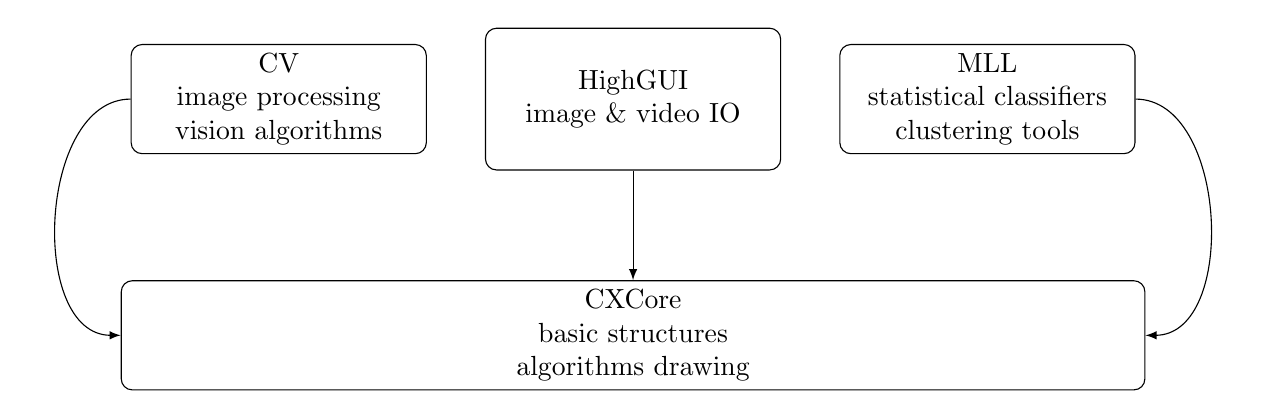
\begin{tikzpicture}
		
		%Nodes
		\node (highGUI) at (0,0) [rectangle, draw, minimum width=2cm, minimum height=1.8cm, 
		align=center, text width=10em, rounded corners]{HighGUI \\ image \& video IO};
		
		\node (CV) at (-4.5,0) [rectangle, draw, minimum width=2cm, minimum height=1cm, 
		align=center, text width=10em, rounded corners]{CV \\ image processing \\ vision 
		algorithms};
		
		\node (MLL) at (4.5,0) [rectangle, draw, minimum width=2cm, minimum height=1cm, 
		align=center, text width=10em, rounded corners]{MLL \\ statistical classifiers \\ 
		clustering tools};
		
		\node (CXCORE) at (0,-3) [rectangle, draw, minimum width=13cm, minimum height=1cm, 
		align=center, text width=10em, rounded corners]{CXCore \\ basic structures \\ algorithms 
		drawing};
		
		%Links
		\draw[-latex] (CV) to [out=180, in=180] (CXCORE);
		\draw[-latex] (highGUI.south) -- (CXCORE.90);
		\draw[-latex] (MLL) to [out=0, in=0] (CXCORE);
		
		\end{tikzpicture}
	}
	\end{center}

\end{figure}

\newpage

%%%%%%%%%%%%%%%%%%%%%%%%%%%%%%%%%%%%%%%%%%%%%%%%%%%%%%%%%%%%%%%%%%%%%%%%%%%%%%%%%%%%%%%%%%%%%%%%%%%%

\section{Example \theblockDiagram}
\stepcounter{blockDiagram}

\begin{figure}[h]
	\begin{center}
		\scalebox{1}{
			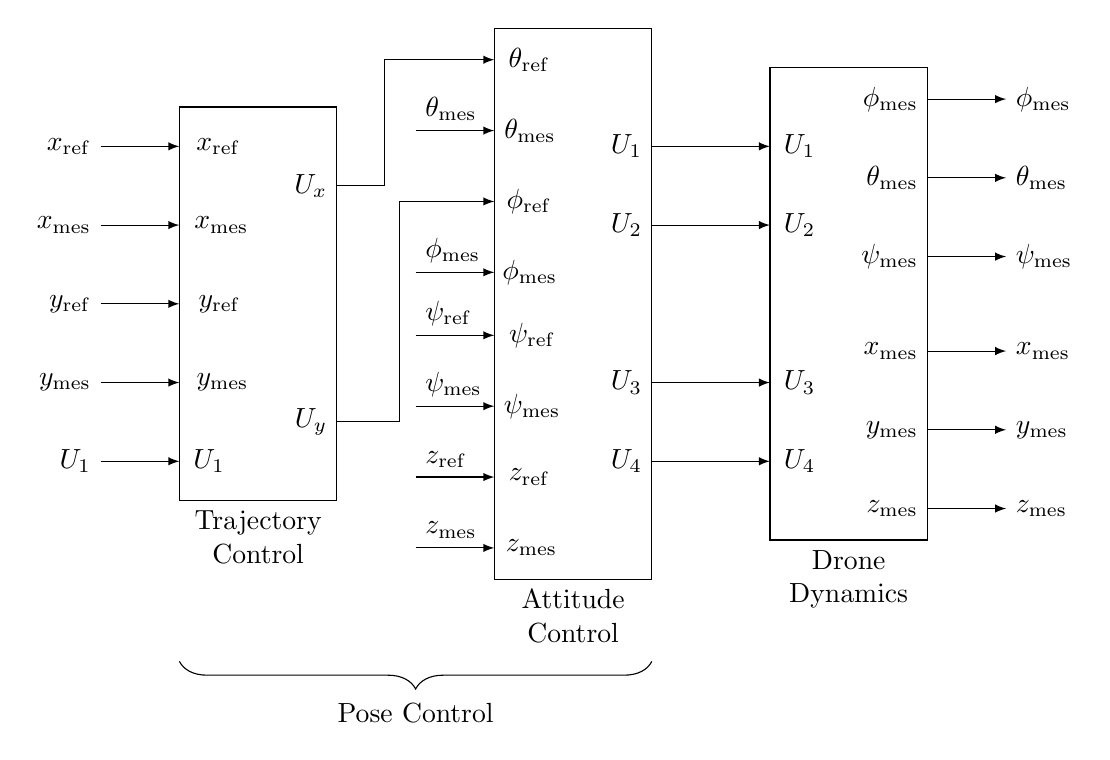
\begin{tikzpicture}
			
			%Trajectory controller
			\node (trajectoryController) at (-4,0) [draw, rectangle, minimum width=2cm, minimum 
			height=5cm, text centered, label={[align=center]below:Trajectory\\ Control}]{};
			
			%Variables
			\draw (-4.1,2.0) coordinate node[left]{$x_\mathrm{ref}$};
			\draw (-4.0,1.0) coordinate node[left]{$x_{\mathrm{mes}}$};
			\draw (-4.1,0.0) coordinate node[left]{$y_\mathrm{ref}$};
			\draw (-4.0,-1.0) coordinate node[left]{$y_{\mathrm{mes}}$};
			\draw (-4.3,-2.0) coordinate node[left]{$U_1$};
			
			\draw (-3.0,1.5) coordinate node[left]{$U_x$};
			\draw (-3.0,-1.5) coordinate node[left]{$U_y$};
			
			%Links
			\draw[-latex] (-6,2.0) coordinate node[left]{$x_\mathrm{ref}$} -- (-5,2.0) coordinate;
			\draw[-latex] (-6,1.0) coordinate node[left]{$x_{\mathrm{mes}}$} -- (-5,1.0) coordinate;
			\draw[-latex] (-6,0.0) coordinate node[left]{$y_\mathrm{ref}$} -- (-5,0.0) coordinate;
			\draw[-latex] (-6,-1.0) coordinate node[left]{$y_{\mathrm{mes}}$} -- (-5,-1.0) 
			coordinate;
			\draw[-latex] (-6,-2.0) coordinate node[left]{$U_1$} -- (-5,-2.0) coordinate; 
			
			
			%Attitude controller
			\node (attitudeController) at (0,0) [draw, rectangle, minimum width=2cm, minimum 
			height=7cm, text centered, label={[align=center]below:Attitude\\ Control}]{};
			
			%Curly brackets
			\draw [decorate,decoration={brace,mirror, amplitude=10pt,raise=4pt},yshift=0pt]
			(-5,-4.4) -- (1,-4.4) node [black,midway,xshift=0.0cm,yshift=-0.8cm] {Pose Control};
			
			%Variables
			\draw (-0.17,3.1) node[left]{$\theta_\mathrm{ref}$};
			\draw (-0.1,2.2) node[left]{$\theta_{\mathrm{mes}}$};
			\draw (-0.15,1.3) node[left]{$\phi_\mathrm{ref}$};
			\draw (-0.08,0.4) node[left]{$\phi_{\mathrm{mes}}$};
			\draw (-0.1,-0.4) node[left]{$\psi_\mathrm{ref}$};
			\draw (-0.04,-1.3) node[left]{$\psi_{\mathrm{mes}}$};
			\draw (-0.17,-2.2) node[left]{$z_\mathrm{ref}$};
			\draw (-0.08,-3.1) node[left]{$z_{\mathrm{mes}}$};
			
			\draw (1.0,2) node[left]{$U_1$};
			\draw (1.0,1) node[left]{$U_2$};
			\draw (1.0,-1) node[left]{$U_3$};
			\draw (1.0,-2) node[left]{$U_4$};
			
			%Links
			\draw[-latex] (-3.0,1.5) coordinate -- (-2.4,1.5) coordinate -- (-2.4,3.1) coordinate  
			-- (-1.0,3.1) coordinate;
			\draw[-latex] (-3,-1.5) -- (-2.2,-1.5) coordinate -- (-2.2,1.3) coordinate -- 
			(-1.0,1.3) coordinate;
			
			\draw[-latex] (-2.0,2.2) coordinate node[above right]{$\theta_{\mathrm{mes}}$} -- 
			(-1.0,2.2) coordinate;
			\draw[-latex] (-2.0,0.4) coordinate node[above right]{$\phi_{\mathrm{mes}}$} -- 
			(-1.0,0.4) coordinate;				
			\draw[-latex] (-2.0,-0.4) coordinate node[above right]{$\psi_\mathrm{ref}$} -- 
			(-1.0,-0.4) coordinate;
			\draw[-latex] (-2.0,-1.3) coordinate node[above right]{$\psi_{\mathrm{mes}}$} -- 
			(-1.0,-1.3) coordinate;	
			\draw[-latex] (-2.0,-2.2) coordinate node[above right]{$z_\mathrm{ref}$} -- (-1.0,-2.2) 
			coordinate;
			\draw[-latex] (-2.0,-3.1) coordinate node[above right]{$z_{\mathrm{mes}}$} -- 
			(-1.0,-3.1) 
			coordinate;	
			
			%Drone model block
			\node (droneMOdel) at (3.5,0) [draw, rectangle, minimum width=2cm, minimum 
			height=6cm, text centered, label={[align=center]below:Drone\\ Dynamics}]{};
			
			%variables
			\draw (3.2,2) coordinate node[left]{$U_1$};
			\draw (3.2,1) coordinate node[left]{$U_2$};
			\draw (3.2,-1) coordinate node[left]{$U_3$};
			\draw (3.2,-2) coordinate node[left]{$U_4$};
			
			\draw (4.5,2.6) coordinate node[left]{$\phi_{\mathrm{mes}}$};
			\draw (4.5,1.6) coordinate node[left]{$\theta_{\mathrm{mes}}$};
			\draw (4.5,0.6) coordinate node[left]{$\psi_{\mathrm{mes}}$};
			\draw (4.5,-0.6) coordinate node[left]{$x_{\mathrm{mes}}$};
			\draw (4.5,-1.6) coordinate node[left]{$y_{\mathrm{mes}}$};
			\draw (4.5,-2.6) coordinate node[left]{$z_{\mathrm{mes}}$};
			
			%Links
			\draw[-latex] (1.0,2) coordinate -- (2.5,2) coordinate;
			\draw[-latex] (1.0,1) coordinate -- (2.5,1) coordinate;
			\draw[-latex] (1.0,-1) coordinate -- (2.5,-1) coordinate;
			\draw[-latex] (1.0,-2) coordinate -- (2.5,-2) coordinate;
			
			\draw[-latex] (4.5,2.6) coordinate -- (5.5,2.6) coordinate 
			node[right]{$\phi_{\mathrm{mes}}$};
			\draw[-latex] (4.5,1.6) coordinate -- (5.5,1.6) coordinate 
			node[right]{$\theta_{\mathrm{mes}}$};
			\draw[-latex] (4.5,0.6) coordinate -- (5.5,0.6) coordinate 
			node[right]{$\psi_{\mathrm{mes}}$};
			\draw[-latex] (4.5,-0.6) coordinate -- (5.5,-0.6) coordinate 
			node[right]{$x_{\mathrm{mes}}$};
			\draw[-latex] (4.5,-1.6) coordinate -- (5.5,-1.6) coordinate 
			node[right]{$y_{\mathrm{mes}}$};
			\draw[-latex] (4.5,-2.6) coordinate -- (5.5,-2.6) coordinate 
			node[right]{$z_{\mathrm{mes}}$};
			
			
			\end{tikzpicture}
		}
	\end{center}
	
\end{figure}

%%%%%%%%%%%%%%%%%%%%%%%%%%%%%%%%%%%%%%%%%%%%%%%%%%%%%%%%%%%%%%%%%%%%%%%%%%%%%%%%%%%%%%%%%%%%%%%%%%%%

\section{Example \theblockDiagram}
\stepcounter{blockDiagram}

\begin{figure}[h]
	\begin{center}	
		\begin{tikzpicture}
		
		%A different way to draw a block diagram
		\bXInput[$\theta_d$]{Reference}               			
		\bXComp*[2]{Comparator}{Reference}              		
		\bXLink{Reference}{Comparator}                  			
		
		\bXBloc[3]{Integrator}{$I$}{Comparator}  					
		\bXLink{Comparator}{Integrator} 							
		\bXComp*[4]{Comparator1}{Integrator}						
		\bXLink{Integrator}{Comparator1}							
		\bXBloc[2]{Proportional}{$P$}{Comparator1}				
		\bXLink{Comparator1}{Proportional}						
		\bXSuma*[4]{Comparator2}{Proportional}				 
		\bXLink{Proportional}{Comparator2}						
		\bXBloc[2]{Integrator1}{$\dfrac{1}{s}$}{Comparator2}		
		\bXLink{Comparator2}{Integrator1}							
		\bXBloc[3]{Integrator2}{$\dfrac{1}{s}$}{Integrator1}		
		\bXLink[$\dot{\theta}$]{Integrator1}{Integrator2}			
		\bXOutput{Uscita}{Integrator2}								
		\bXLink[$\theta$]{Integrator2}{Uscita}						
		\bXReturn[5]{Integrator2-Uscita}{Comparator}{}			
		\bXReturn{Integrator1-Integrator2}{Comparator1}{}	    
		\bXBranchy[-4]{Comparator-Integrator}{Proportional2}	
		\bXChain[1.5]{Proportional2}{p/$P$}						
		\bXLinkyx{Comparator-Integrator}{p}						
		\bXLinkxy{p}{Comparator2}								
		
		\end{tikzpicture}
	\end{center}
\end{figure}

\newpage

%%%%%%%%%%%%%%%%%%%%%%%%%%%%%%%%%%%%%%%%%%%%%%%%%%%%%%%%%%%%%%%%%%%%%%%%%%%%%%%%%%%%%%%%%%%%%%%%%%%%

\section{Example \theblockDiagram}
\stepcounter{blockDiagram}

\begin{figure}[h]
	\begin{center}
		\scalebox{0.75}{
			\begin{tikzpicture}
						
			\node (pd1) at (0,0) [draw, rectangle, text centered, minimum width=1.5cm, minimum 
			height=1cm]{$\text{PD}_\theta$};
			
			\node (adder1) at (-2,0) [draw, circle, text centered, minimum size=0.5cm]{};
			
			\draw[-latex] (-2,-1.5) coordinate node[below]{$\theta_{\mathrm{mes}}$} -- 
			(adder1.south);
			\draw[-latex] (adder1.east) node[above right]{$e_\theta$} -- (pd1.west);
			\draw[-latex] (-3,0) coordinate node[left]{$\theta_\mathrm{ref}$}-- (adder1.west);
			
			\draw (-2.05,0.15) coordinate node[above left]{$+$};
			\draw (-2.05,-0.25) coordinate node[below right]{$-$};
			
			\node (pd2) at (0,-3.0) [draw, rectangle, text centered, minimum width=1.5cm, minimum 
			height=1cm]{$\text{PD}_\phi$};
			
			\node (adder2) at (-2,-3.0) [draw, circle, text centered, minimum size=0.5cm]{};
			
			\draw[-latex] (-2,-4.5) coordinate node[below]{$\phi_{\mathrm{mes}}$} -- (adder2.south);
			\draw[-latex] (adder2.east) node[above right]{$e_\phi$} -- (pd2.west);
			\draw[-latex] (-3,-3) coordinate node[left]{$\phi_\mathrm{ref}$} -- (adder2.west);
			
			\draw (-2.05,-2.85) coordinate node[above left]{$+$};
			\draw (-2.05,-3.25) coordinate node[below right]{$-$};
			
			\node (pd3) at (0,-6.0) [draw, rectangle, text centered, minimum width=1.5cm, minimum 
			height=1cm]{$\text{PD}_\psi$};
			
			\node (adder3) at (-2,-6.0) [draw, circle, text centered, minimum size=0.5cm]{};
			
			\draw[-latex] (-2,-7.5) coordinate node[below]{$\psi_{\mathrm{mes}}$} -- (adder3.south);
			\draw[-latex] (adder3.east) node[above right]{$e_\psi$} -- (pd3.west);
			\draw[-latex] (-3,-6) coordinate node[left]{$\psi_\mathrm{ref}$} -- (adder3.west);
			
			\draw (-2.05,-5.85) coordinate node[above left]{$+$};
			\draw (-2.05,-6.25) coordinate node[below right]{$-$};
			
			\node (pd4) at (0,-9.0) [draw, rectangle, text centered, minimum width=1.5cm, minimum 
			height=1cm]{$\text{PD}_z$};
			
			\node (adder4) at (-2,-9.0) [draw, circle, text centered, minimum size=0.5cm]{};
			
			\draw[-latex] (-2,-10.5) coordinate node[below]{$z_{\mathrm{mes}}$} -- (adder4.south);
			\draw[-latex] (adder4.east) node[above right]{$e_z$} -- (pd4.west);
			\draw[-latex] (-3,-9) coordinate node[left]{$z_\mathrm{ref}$} -- (adder4.west);
			
			\draw (-2.05,-8.85) coordinate node[above left]{$+$};
			\draw (-2.05,-9.25) coordinate node[below right]{$-$};
			
			
			\node (droneModel) at (3,-4.5) [draw, rectangle, minimum height=11cm, minimum 
			width=2cm, text centered, text 		
			width=1em]{D\\R\\O\\N\\E\\$\hspace{0.1cm}$\\M\\O\\D\\E\\L\\};
			
			\draw[-latex] (pd1.east) node [above right]{$U_3$} -- (2.0,0.0) coordinate;
			\draw[-latex] (pd2.east) node [above right]{$U_2$} -- (2.0,-3.0) coordinate;
			\draw[-latex] (pd3.east) node [above right]{$U_4$} -- (2.0,-6.0) coordinate;
			\draw[-latex] (pd4.east) node [above right]{$U_1$} -- (2.0,-9.0) coordinate;
			
			\draw[-latex] (4.0,0) coordinate -- (5,0) coordinate 
			node[right]{$\theta_{\mathrm{mes}}$};
			\draw[-latex] (4.0,-3) coordinate -- (5,-3) coordinate 
			node[right]{$\phi_{\mathrm{mes}}$};
			\draw[-latex] (4.0,-6) coordinate -- (5,-6) coordinate 
			node[right]{$\psi_{\mathrm{mes}}$};
			\draw[-latex] (4.0,-9) coordinate -- (5,-9) coordinate node[right]{$z_{\mathrm{mes}}$};
			
			
			\end{tikzpicture}
		}
	\end{center}
	
\end{figure}

%%%%%%%%%%%%%%%%%%%%%%%%%%%%%%%%%%%%%%%%%%%%%%%%%%%%%%%%%%%%%%%%%%%%%%%%%%%%%%%%%%%%%%%%%%%%%%%%%%%%

\section{Example \theblockDiagram}
\stepcounter{blockDiagram}

\begin{figure}[h]
	\begin{center}
		\scalebox{0.8}{
			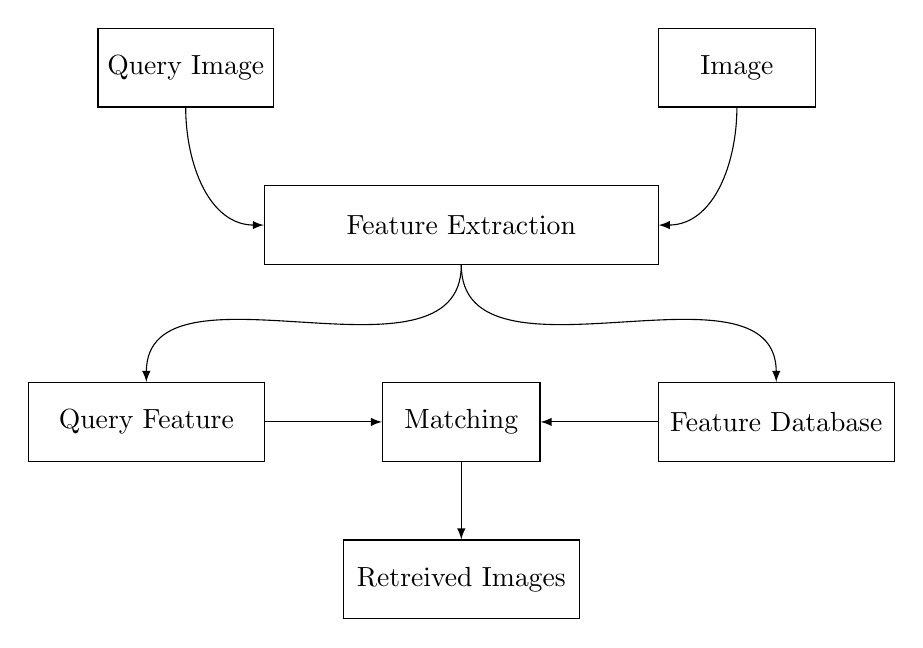
\begin{tikzpicture}[node distance=2cm]
			
			%Nodes	
			\node (queryImage) at (-3.5, 0) [rectangle, draw, text centered, minimum width=2cm, 
			minimum height=1cm] {Query Image};
			
			\node (image) at ( 3.5, 0) [rectangle, text centered, draw, minimum width=2cm, minimum 
			height=1cm] {Image};
			
			\node (featureExtraction) at ( 0,-2) [rectangle, draw, text centered, minimum 
			width=5cm, minimum height=1cm] {Feature Extraction};
			
			\node (queryFeature) at (-4,-4.5) [rectangle, draw, text centered, minimum width=3cm, 
			minimum height=1cm] {Query Feature};
			
			\node (matching) at ( 0,-4.5) [rectangle, draw, text centered, minimum width=2cm, 
			minimum height=1cm] {Matching};
			
			\node (featureDatabase) at ( 4,-4.5) [rectangle, draw, text centered, minimum 
			width=3cm, minimum height=1cm] {Feature Database};
			
			\node (retreivedImages) at ( 0,-6.5) [rectangle, draw, text centered, minimum 
			width=3cm, minimum height=1cm] {Retreived Images};
			
			%Links
			\draw [-latex] (queryFeature.east) -- (matching.west);
			\draw [-latex] (featureDatabase.west) -- (matching.east);
			\draw [-latex] (matching.south) -- (retreivedImages.north);
			\draw [-latex] (queryImage) to [out=270,in=180] (featureExtraction);
			\draw [-latex] (image) to [out=270,in=0] (featureExtraction);
			\draw [-latex] (featureExtraction) to [out=270,in=90] (queryFeature);
			\draw [-latex] (featureExtraction) to [out=270,in=90] (featureDatabase);
			
			\end{tikzpicture}
		}
	\end{center}
\end{figure}

\newpage

%%%%%%%%%%%%%%%%%%%%%%%%%%%%%%%%%%%%%%%%%%%%%%%%%%%%%%%%%%%%%%%%%%%%%%%%%%%%%%%%%%%%%%%%%%%%%%%%%%%%

\section{Example \theblockDiagram}
\stepcounter{blockDiagram}

\begin{figure}[h]
	\begin{center}
		\scalebox{0.95}{
		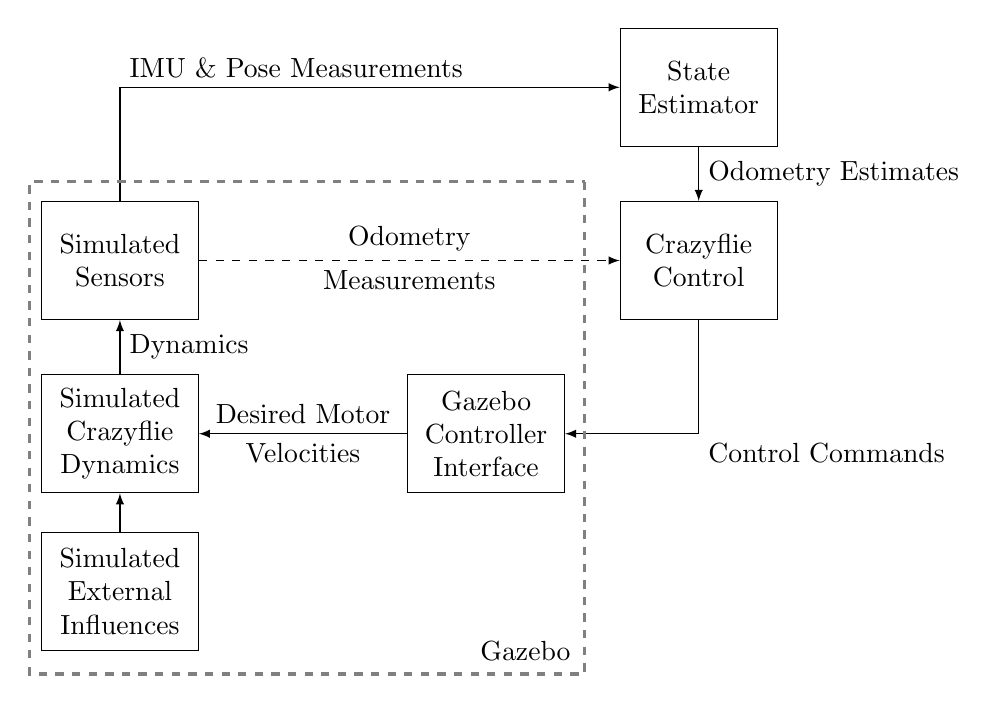
\begin{tikzpicture}
		
		%Blocks
		\node (CrazyflieControl) at (0.2,0) [draw, rectangle, minimum width=1.5cm, minimum 
		height=1.5cm, text centered, text width=5em]{Crazyflie Control};
		\node (GazeboControllerInterface) at (-2.5,-2.2) [draw, rectangle, minimum width=1.5cm, 
		minimum height=1.5cm, text centered, text width=5em]{Gazebo Controller\\Interface};
		\node (SimulatedExternalInfluence) at (-7.15,-4.2) [draw, rectangle, minimum 
		width=1.5cm, minimum height=1.5cm, text centered, text width=5em]{Simulated 
		External\\Influences};
		\node (SimulatedCrazyflieDynamics) at (-7.15,-2.2) [draw, rectangle, minimum 
		width=1.5cm, minimum height=1.5cm, text centered, text width=5em]{Simulated 
		Crazyflie\\Dynamics};
		\node (SimulatedSensor) at (-7.15,0) [draw, rectangle, minimum width=1.5cm, minimum 
		height=1.5cm, text centered, text width=5em]{Simulated Sensors};
		\node (StateEstimator) at (0.2,2.2) [draw, rectangle, minimum width=1.5cm, minimum 
		height=1.5cm, text centered, text width=5em]{State Estimator};
		
		%Links
		\draw[-latex] (CrazyflieControl) |- node[below right]{Control Commands} 
		(GazeboControllerInterface);
		\draw[-latex] (GazeboControllerInterface) -- node[above]{Desired Motor} 
		node[below]{Velocities} (SimulatedCrazyflieDynamics);
		\draw[-latex] (SimulatedExternalInfluence) -- (SimulatedCrazyflieDynamics);
		\draw[-latex] (SimulatedSensor) |- node[above right]{IMU \& Pose Measurements} 
		(StateEstimator);
		\draw[-latex] (StateEstimator) -- node[right]{Odometry Estimates} (CrazyflieControl);
		\draw[-latex] (SimulatedCrazyflieDynamics) -- node[right] {Dynamics} (SimulatedSensor);
		\draw[-latex, dashed] (SimulatedSensor) -- node[above]{Odometry} 
		node[below]{Measurements} (CrazyflieControl) ;
		
		%Gazebo's group
		\draw[dashed, gray, draw, line width=1.25pt] (-1.25,1) coordinate -- (-1.25,-5.25) 
		coordinate -- (-8.3,-5.25) coordinate -- (-8.3,1) coordinate -- (-1.25,1) coordinate; 
		\draw (-2,-5.2) coordinate node[above]{Gazebo};
		
		\end{tikzpicture}
	}
	\end{center}
\end{figure}

%%%%%%%%%%%%%%%%%%%%%%%%%%%%%%%%%%%%%%%%%%%%%%%%%%%%%%%%%%%%%%%%%%%%%%%%%%%%%%%%%%%%%%%%%%%%%%%%%%%%

\section{Example \theblockDiagram}
\stepcounter{blockDiagram}

\begin{figure}[h]
	\begin{center}
		\scalebox{0.9}{
			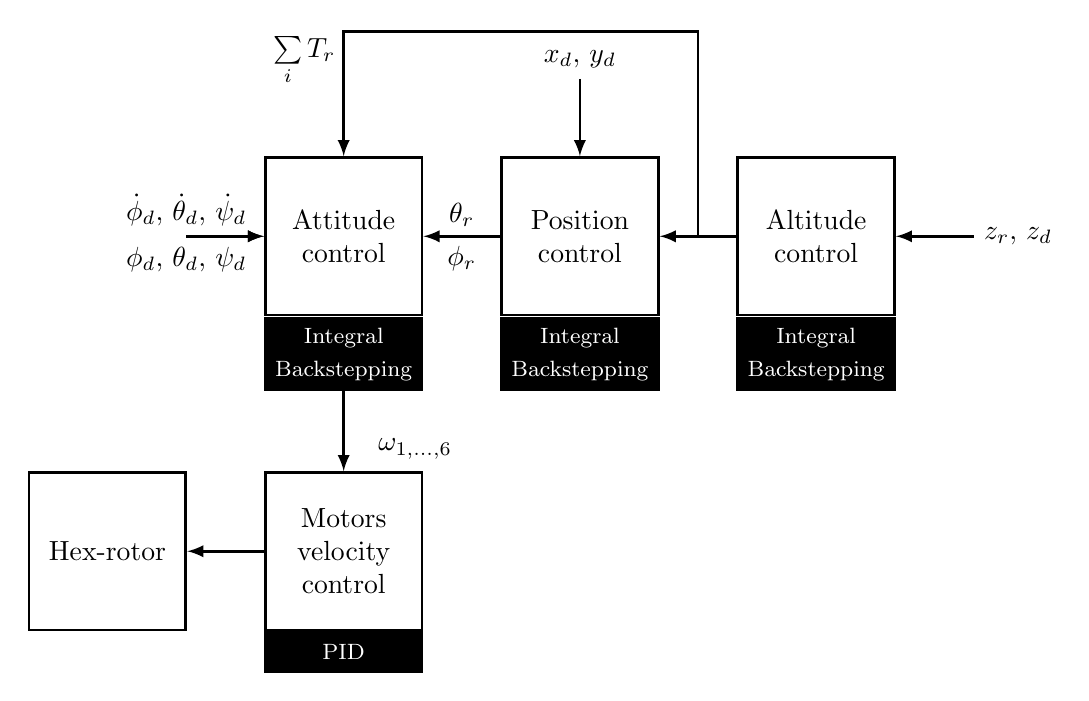
\begin{tikzpicture}
			
			%Attitude controller
			\node (attitudeController) at (-3,0) [draw, rectangle, text centered, line width=1.0pt, 
			minimum height=2cm, minimum width=1cm, text width=5em]{Attitude\\ control};
			
			%baseline Integral Backstepping
			\node (baselineIntegralBackstepping) at (-3,-1.50) [draw, line width=1.0pt, fill=black, 
			rectangle, minimum height=0.5cm, minimum width=1cm, text centered, text 
			width=5em]{\footnotesize{\color{white}{Integral\\ Backstepping}}}; 
			
			%PositionController
			\node (positionController) at (0,0) [draw, rectangle, line width=1.0pt, text centered, 
			minimum height=2cm, minimum width=1cm, text width=5em]{Position\\ control};
			
			%Baseline Integral Backstepping
			\node at (0,-1.50) [draw, line width=1.0pt, fill=black, rectangle, minimum 
			height=0.5cm, minimum width=1cm, text centered, text 
			width=5em]{\footnotesize{\color{white}{Integral\\ Backstepping}}}; 
			
			%Altitude controller
			\node (altitudeController) at (3,0) [draw, rectangle, line width=1.0pt, text centered, 
			minimum height=2cm, minimum width=1cm, text width=5em]{Altitude\\ control};
			
			%Baseline Integral Backstepping
			\node at (3,-1.50) [draw, line width=1.0pt, fill=black, rectangle, minimum 
			height=0.5cm, minimum width=1cm, text centered, text 
			width=5em]{\footnotesize{\color{white}{Integral\\ Backstepping}}}; 
			
			%Motors controller
			\node (motorsController) at (-3,-4) [draw, rectangle, line width=1.0pt, text 
			centered, minimum height=2cm, minimum width=1cm, text width=5em]{Motors velocity 
			control};
			
			%Baseline PID
			\node at (-3,-5.28) [draw, line width=1.0pt, fill=black, rectangle, minimum 
			height=0.5cm, minimum width=1cm, text centered, text 
			width=5em]{\footnotesize{\color{white}{PID}}}; 
			
			%Hexarotor
			\node (hexarotor) at (-6,-4) [draw, rectangle, line width=1.0pt, text centered, 
			minimum height=2cm, minimum width=1cm, text width=5em]{Hex-rotor};
			
			%Links
			\draw[-latex, line width=1.0pt] (motorsController.west) -- (hexarotor.east);
			\draw[-latex, line width=1.0pt] (altitudeController.west) -- (positionController.east);
			\draw[-latex, line width=1.0pt] (positionController.west) -- (attitudeController.east);
			\draw[-latex, line width=1.0pt] (baselineIntegralBackstepping.south) -- 
			(motorsController.north);
			
			\draw[-latex, line width=1.0pt] (1.5,0) coordinate -- (1.5,2.6) coordinate -- (-3,2.6) 
			coordinate -- (attitudeController.north);
			
			%Reference signals
			\draw[-latex, line width=1.0pt] (5,0) coordinate node[right]{$z_r,\,z_d$}-- 
			(altitudeController.east);
			\node[above] at (-3.5,1.8) [text centered]{$\sum\limits_i T_r$};
			\draw[-latex, line width=1.0pt] (0,2) coordinate node[above]{$x_d,\,y_d$} -- 
			(positionController.north);
			\node[above] at (-1.5,0) [text centered]{$\theta_r$};
			\node[below] at (-1.5,0) [text centered]{$\phi_r$};
			\draw[-latex, line width=1.0pt] (-5.0,0) coordinate 
			node[below]{$\phi_d,\,\theta_d,\,\psi_d$} -- (attitudeController.west);
			\draw[-latex, line width=1.0pt] (-5.0,0) coordinate 
			node[above]{$\dot{\phi}_d,\,\dot{\theta}_d,\,\dot{\psi}_d$} -- 
			(attitudeController.west);
			\node at (-1.5,-2.7) [left, text centered]{$\omega_{1,\dots,6}$}; 
			
			\end{tikzpicture}
		}
	\end{center}
	
	
\end{figure}

\newpage

%%%%%%%%%%%%%%%%%%%%%%%%%%%%%%%%%%%%%%%%%%%%%%%%%%%%%%%%%%%%%%%%%%%%%%%%%%%%%%%%%%%%%%%%%%%%%%%%%%%%

\section{Example \theblockDiagram}
\stepcounter{blockDiagram}

\begin{figure}[h]
	\begin{center}
		\begin{tikzpicture}[node distance=2cm]
		
		%Creo i nodi del diagramma di flusso		
		\node (allSubWindow) at (-3,1) [ellipse, draw, text centered, text width=6em] {All 
		sub-windows};
		
		\node (furtherProcessing) at (3,1) [ellipse, draw, text centered, text width=6em] {Further 
		Elaboration};
		
		\node (1) at (-3,-1.25) [circle, draw, text centered, minimum size=1.2cm] {1};
		
		\node (2) at (0,-1.25) [circle, draw, text centered, minimum size=1.2cm] {2};
		
		\node (3) at (3,-1.25) [circle, draw, text centered, minimum size=1.2cm] {3};
		
		\node (rejectSubWindows) at (0,-4.25) [ellipse, draw, text centered, text width=6em] 
		{Sub-windows rejection};
		
		\draw[-latex] (1) -- node[above]{T} (2);
		\draw[-latex] (2) -- node[above]{T} (3);
		\draw[-latex] (2) -- node[above left]{F} (rejectSubWindows);
		\draw[-latex] (1) -- node[above right]{F} (rejectSubWindows);
		\draw[-latex] (3) -- node[above left]{F} (rejectSubWindows);
		\draw[-latex] (allSubWindow) to [out=200,in=180] (1);
		\draw[-latex] (3) to [out=0, in=340] (furtherProcessing);
		
		\end{tikzpicture}
	\end{center}
	
\end{figure}

%%%%%%%%%%%%%%%%%%%%%%%%%%%%%%%%%%%%%%%%%%%%%%%%%%%%%%%%%%%%%%%%%%%%%%%%%%%%%%%%%%%%%%%%%%%%%%%%%%%%

\section{Example \theblockDiagram}
\stepcounter{blockDiagram}

\begin{figure}[h]
	\begin{center}
		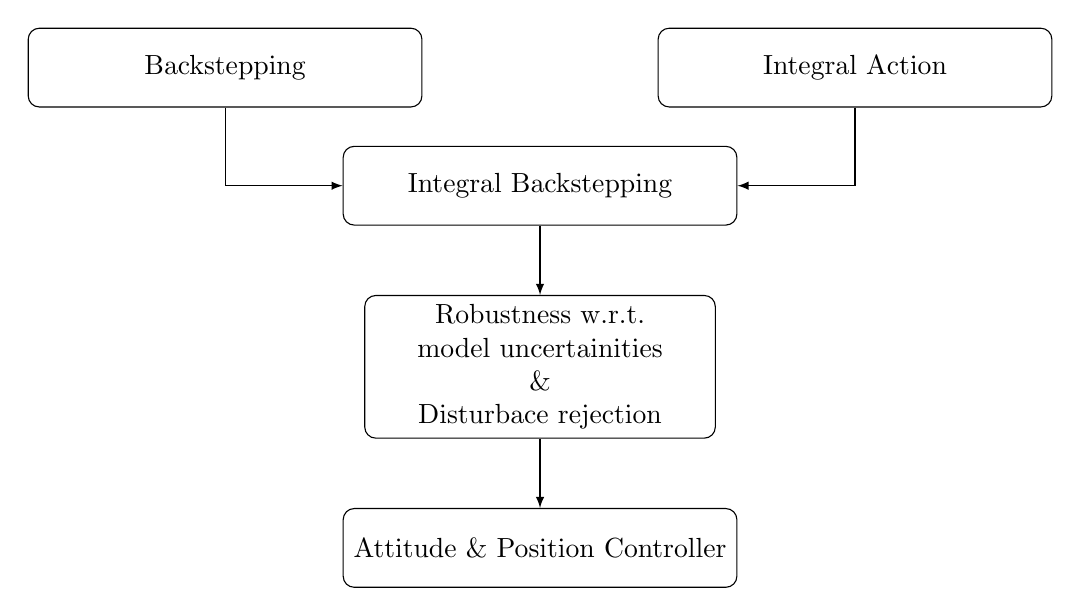
\begin{tikzpicture}
		
		%Nodes
		\node (BackStepping) at (-4,1.5) [draw, rectangle, minimum height=1cm, minimum width=5cm, 
		text centered, rounded corners]{Backstepping};
		\node (integralAction) at (4,1.5) [draw, rectangle, minimum height=1cm, minimum width=5cm, 
		text centered, rounded corners]{Integral Action};
		
		%Rappresento il nodo centrale
		\node (integralBackStepping) at (0,0) [draw, rectangle, minimum height=1cm, minimum 
		width=5cm, text centered, rounded corners]{Integral Backstepping};
		
		%Rappresento il blocco caratteristiche
		\node (features) at (0,-2.3) [draw, rectangle, minimum height=1cm, minimum 
		width=1cm, text centered, rounded corners, text width=12em]{Robustness w.r.t. model 
		uncertainities\\ \& \\Disturbace rejection};
		
		%Control system results
		\node (results) at (0,-4.6) [draw, rectangle, minimum height=1cm, minimum width=5cm, text 
		centered, rounded corners]{Attitude \& Position Controller};
		
		%Links
		\draw[-latex] (BackStepping.270) -- (-4,0) coordinate -- (integralBackStepping.180);
		\draw[-latex] (integralAction.270) -- (4,0) coordinate -- (integralBackStepping.0);
		\draw[-latex] (integralBackStepping.south) -- (features.north);
		\draw[-latex] (features.south) -- (results.north);
		
		
		\end{tikzpicture}
	\end{center}
	
\end{figure}

\newpage

%%%%%%%%%%%%%%%%%%%%%%%%%%%%%%%%%%%%%%%%%%%%%%%%%%%%%%%%%%%%%%%%%%%%%%%%%%%%%%%%%%%%%%%%%%%%%%%%%%%%

\section{Example \theblockDiagram}
\stepcounter{blockDiagram}

\begin{figure}[h]
	\begin{center}
		\scalebox{0.8}{
		\begin{tikzpicture}
		
		%System nodes
		\node [rectangle, draw, text width=6em, text centered, rounded corners, minimum height=4em] 
		(start) at (0,0) {START};
		
		\node [rectangle, draw, text width=6em, text centered, rounded corners, minimum height=4em, 
		below of=init] (vrMatlab) at (0,-1.5) {VR MATLAB};
		
		\node [rectangle, draw, text width=6em, text centered, rounded corners, minimum height=4em, 
		below of=identify] (detection) at (0,-4.0) {DETECTION};
		
		\node [rectangle, draw, text width=6em, text centered, rounded corners, minimum height=4em, 
		left of=evaluate, node distance=3cm] (update) at (-1.5,-5) {UPDATE UAV POSE};
		
		\node [diamond, draw, text width=5.5em, text badly centered, node distance=3cm, inner 
		sep=0pt, below of=evaluate] (decide) at (0,-5.5) {CAR DETECTED?};
		
		
		%Links
		\path [draw, -latex'] (start) -- (vrMatlab);
		\path [draw, -latex'] (vrMatlab) -- (detection);
		\path [draw, -latex'] (detection) -- (decide);
		\path [draw, -latex'] (decide) -| (update);
		\path [draw, -latex'] (update) |- (vrMatlab);
		\path [draw, -latex'] (decide.east) -- (4.5,-8.5) coordinate -- (4.5,-2.5) coordinate -- 
		(vrMatlab.east);
		
		%Decisions
		\node at (2.5,-8.5)  [above] {NO};
		\node at (-2.5,-8.5) [above] {YES};
		
		\end{tikzpicture}
	}
	\end{center}
	
\end{figure}

%%%%%%%%%%%%%%%%%%%%%%%%%%%%%%%%%%%%%%%%%%%%%%%%%%%%%%%%%%%%%%%%%%%%%%%%%%%%%%%%%%%%%%%%%%%%%%%%%%%%

\section{Example \theblockDiagram}
\stepcounter{blockDiagram}

\begin{figure}[h]
	\begin{center}
		\scalebox{1}{
			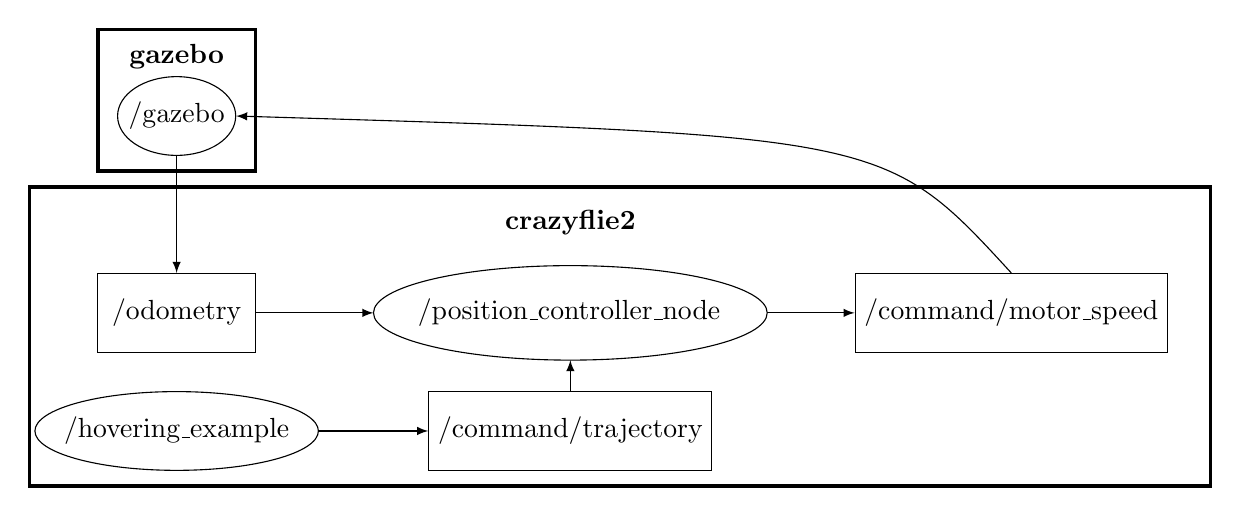
\begin{tikzpicture}
			
			%Nodes
			\draw (0,1.5) ellipse (1.8cm and 0.5cm) node[] {/hovering\_example};
			\draw (5,3) ellipse (2.5cm and 0.6cm);
			\draw (5.7,3) node[text width=15em]{/position\_controller\_node};
			\draw (0,5.5) ellipse (0.75cm and 0.5cm) node[]{/gazebo};
			
			%Topics
			\node (commandTrajectory) at (5,1.5) [draw, text centered, rectangle, minimum 
			height=1cm]{/command/trajectory};
			\node (odometrySensor) at (0,3) [draw, rectangle, minimum height=1cm, text centered, 
			minimum width=2cm]{/odometry};
			\node (motorSpeed) at (10.6,3) [draw, rectangle, minimum height=1cm, text 
			centered]{/command/motor\_speed};
			
			%Links
			\draw[-latex] (1.8,1.5) coordinate -- (commandTrajectory);
			\draw[-latex] (odometrySensor) -- (2.5,3) coordinate;
			\draw[-latex] (7.5,3) coordinate -- (motorSpeed.west);
			\draw[-latex] (commandTrajectory) -- (5,2.4) coordinate;
			\draw[-latex] (0,5) coordinate -- (odometrySensor.north);
			\draw[-latex] (motorSpeed.north) .. controls (9,5.25) .. (0.755,5.5);
			
			%Crazyflie 2.0 box
			\node (crazyflie) at (5.63,2.7) [draw, rectangle, line width=1.25 pt, minimum 
			height=3.8cm, minimum width=15cm]{};
			\draw (5,4.15) coordinate node[]{\textbf{crazyflie2}};
			
			%Rettangolo che raffigura gazebo
			\node (gazeboBox) at (0,5.7) [draw, rectangle, line width=1.25 pt, minimum 
			height=1.8cm, minimum width=2cm]{};
			\draw (0, 6.25) coordinate node[]{\textbf{gazebo}};
			
			\end{tikzpicture}
		}
	\end{center}
\end{figure} 

\newpage

%%%%%%%%%%%%%%%%%%%%%%%%%%%%%%%%%%%%%%%%%%%%%%%%%%%%%%%%%%%%%%%%%%%%%%%%%%%%%%%%%%%%%%%%%%%%%%%%%%%%

\section{Example \theblockDiagram}
\stepcounter{blockDiagram}

\begin{figure}[h]
	\begin{center}
		\scalebox{0.75}{
		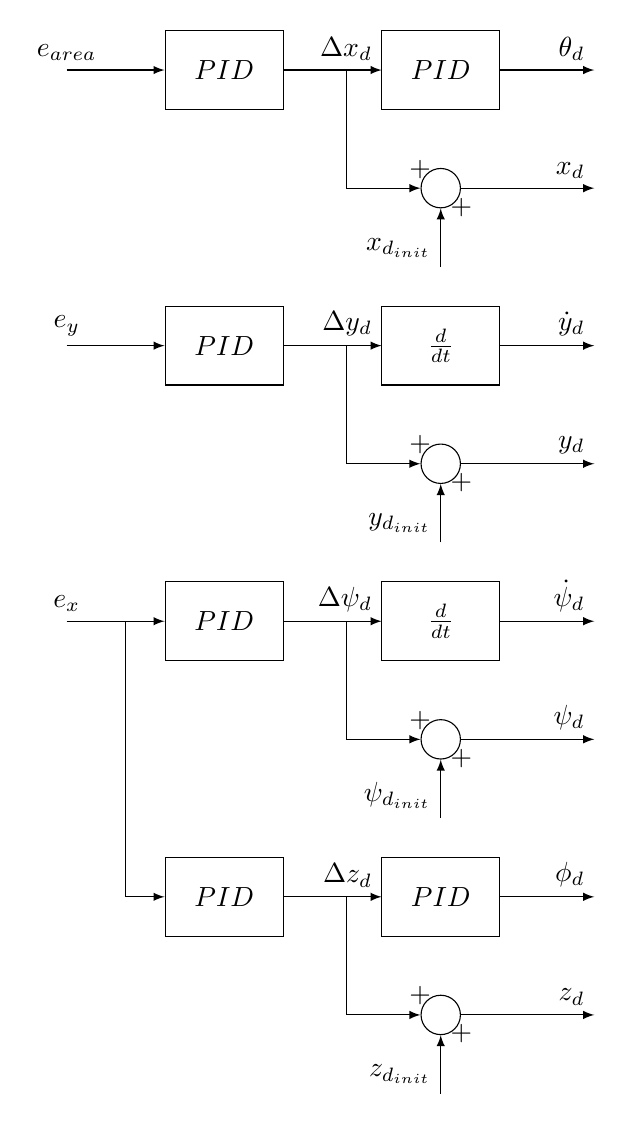
\begin{tikzpicture}
		
		%Nodes
		\node (firstPID) at (-2,0.5) [draw, rectangle, minimum width=1.5cm, minimum height=1cm, 
		text centered]{$PID$};
		
		\node (secondPID) at (0.75,0.5) [draw, text centered, minimum width=1.5cm, minimum 
		height=1cm]{$PID$};
		
		\node (adder) at (0.75,-1) [draw, circle, text centered, minimum size=0.5cm]{};
		
		%Links
		\draw[-latex] (-4,0.5) coordinate node[above]{$e_{area}$} -- (firstPID.west);
		
		\draw[-latex] (firstPID.east) -- (0,0.5) coordinate node[above left]{$\Delta x_d$};
		
		\draw[-latex] (secondPID.east) -- (2.7,0.5) coordinate node[above left]{$\theta_d$};
		
		\draw[-latex] (-0.45,0.5) coordinate -- (-0.45,-1) coordinate -- (adder.west);
		
		\draw[-latex] (adder.east) -- (2.7,-1) coordinate node[above left]{$x_d$};
		
		\draw[-latex] (0.75,-2.0) coordinate node[above left]{$x_{d_{init}}$} -- (adder.south);
		
		%Signs
		\draw (0.75,-1) coordinate node[above left]{$+$};
		\draw (0.75,-1) coordinate node[below right]{$+$};
		
		%Names into the second part of the scheme
		\node (thirdPID) at (-2,-3.0) [draw, rectangle, minimum width=1.5cm, minimum height=1cm, 
		text centered]{$PID$};
		
		\node (fourthPID) at (0.75,-3.0) [draw, text centered, minimum width=1.5cm, minimum 
		height=1cm]{$\frac{d}{dt}$};
		
		\node (adder1) at (0.75,-4.5) [draw, circle, text centered, minimum size=0.5cm]{};
		
		%Links among blocks
		\draw[-latex] (-4,-3.0) coordinate node[above]{$e_y$} -- (thirdPID.west);
		
		\draw[-latex] (thirdPID.east) -- (0,-3.0) coordinate node[above left]{$\Delta y_d$};
		
		\draw[-latex] (fourthPID.east) -- (2.7,-3.0) coordinate node[above left]{$\dot{y}_d$};
		
		\draw[-latex] (-0.45,-3.0) coordinate -- (-0.45,-4.5) coordinate -- (adder1.west);
		
		\draw[-latex] (adder1.east) -- (2.7,-4.5) coordinate node[above left]{$y_d$};
		
		\draw[-latex] (0.75,-5.5) coordinate node[above left]{$y_{d_{init}}$} -- (adder1.south);
		
		%Signs
		\draw (0.75,-4.5) coordinate node[above left]{$+$};
		\draw (0.75,-4.5) coordinate node[below right]{$+$};
		
		%Third part of the scheme
		\node (fifthPID) at (-2,-6.5) [draw, rectangle, minimum width=1.5cm, minimum height=1cm, 
		text centered]{$PID$};
		
		\node (sixthPID) at (0.75,-6.5) [draw, text centered, minimum width=1.5cm, minimum 
		height=1cm]{$\frac{d}{dt}$};
		
		\node (adder2) at (0.75,-8.0) [draw, circle, text centered, minimum size=0.5cm]{};
		
		%Links among blocks
		\draw[-latex] (-4,-6.5) coordinate node[above]{$e_x$} -- (fifthPID.west);
		
		\draw[-latex] (fifthPID.east) -- (0,-6.5) coordinate node[above left]{$\Delta \psi_d$};
		
		\draw[-latex] (sixthPID.east) -- (2.7,-6.5) coordinate node[above left]{$\dot{\psi}_d$};
		
		\draw[-latex] (-0.45,-6.5) coordinate -- (-0.45,-8.0) coordinate -- (adder2.west);
		
		\draw[-latex] (adder2.east) -- (2.7,-8.0) coordinate node[above left]{$\psi_d$};
		
		\draw[-latex] (0.75,-9.0) coordinate node[above left]{$\psi_{d_{init}}$} -- 
		(adder2.south);
		
		%Signs
		\draw (0.75,-8.0) coordinate node[above left]{$+$};
		\draw (0.75,-8.0) coordinate node[below right]{$+$};
		
		
		%Signs
		\node (seventhPID) at (-2,-10) [draw, rectangle, minimum width=1.5cm, minimum height=1cm, 
		text centered]{$PID$};
		
		\node (eighthPID) at (0.75,-10) [draw, text centered, minimum width=1.5cm, minimum 
		height=1cm]{$PID$};
		
		\node (adder3) at (0.75,-11.5) [draw, circle, text centered, minimum size=0.5cm]{};
		
		%Links
		\draw[-latex] (-3.25,-6.5) coordinate -- (-3.25,-10) coordinate -- (seventhPID.west);
		
		\draw[-latex] (seventhPID.east) -- (0,-10) coordinate node[above left]{$\Delta z_d$};
		
		\draw[-latex] (eighthPID.east) -- (2.7,-10) coordinate node[above left]{$\phi_d$};
		
		\draw[-latex] (-0.45,-10) coordinate -- (-0.45,-11.5) coordinate -- (adder3.west);
		
		\draw[-latex] (adder3.east) -- (2.7,-11.5) coordinate node[above left]{$z_d$};
		
		\draw[-latex] (0.75,-12.5) coordinate node[above left]{$z_{d_{init}}$} -- (adder3.south);
		
		%Signs
		\draw (0.75,-11.5) coordinate node[above left]{$+$};
		\draw (0.75,-11.5) coordinate node[below right]{$+$};
		\end{tikzpicture}
	}
	\end{center}
	
\end{figure}

%%%%%%%%%%%%%%%%%%%%%%%%%%%%%%%%%%%%%%%%%%%%%%%%%%%%%%%%%%%%%%%%%%%%%%%%%%%%%%%%%%%%%%%%%%%%%%%%%%%%

\section{Example \theblockDiagram}
\stepcounter{blockDiagram}

\begin{figure}[h]
	\begin{center}
		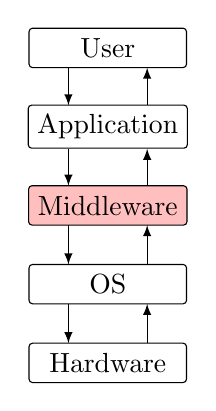
\begin{tikzpicture}
		
		%Layer architecture
		\node (user) at (0,0) [rectangle, draw, rounded corners=1.25pt, text centered, minimum 
		width=2cm, minimum height=0.5cm]{User};
		
		\node (application) at (0,-1) [rectangle, draw, rounded corners=1.25pt, text centered, 
		minimum width=2cm, minimum height=0.5cm]{Application};
		
		\node (middleware) at (0,-2) [rectangle, draw, rounded corners=1.25pt, text centered, 
		minimum width=2cm, fill=red!25, minimum height=0.5cm]{Middleware};
		
		\node (OS) at (0,-3) [rectangle, draw, rounded corners=1.25pt, text centered, minimum 
		width=2cm, minimum height=0.5cm]{OS};
		
		\node (hardware) at (0,-4) [rectangle, draw, rounded corners=1.25pt, text centered, minimum 
		width=2cm, minimum height=0.5cm]{Hardware};
		
		%RLinks
		\draw[-latex] (-0.5, -0.25) to (-0.5,-0.73);
		\draw[latex-] (0.5, -0.25) to (0.5,-0.73);
		
		\draw[-latex] (-0.5,-1.28) to (-0.5,-1.75);
		\draw[latex-] (0.5,-1.28) to (0.5,-1.75);
		
		\draw[-latex] (-0.5,-2.25) to (-0.5,-2.75);
		\draw[latex-] (0.5,-2.25) to (0.5,-2.75);
		
		\draw[-latex] (-0.5,-3.25) to (-0.5,-3.75);
		\draw[latex-] (0.5,-3.25) to (0.5,-3.75);
		
		\end{tikzpicture}
	\end{center}
\end{figure}

\newpage

%%%%%%%%%%%%%%%%%%%%%%%%%%%%%%%%%%%%%%%%%%%%%%%%%%%%%%%%%%%%%%%%%%%%%%%%%%%%%%%%%%%%%%%%%%%%%%%%%%%%

\section{Example \theblockDiagram}
\stepcounter{blockDiagram}

\begin{figure}[h]
	\begin{center}
		\scalebox{0.9}{
			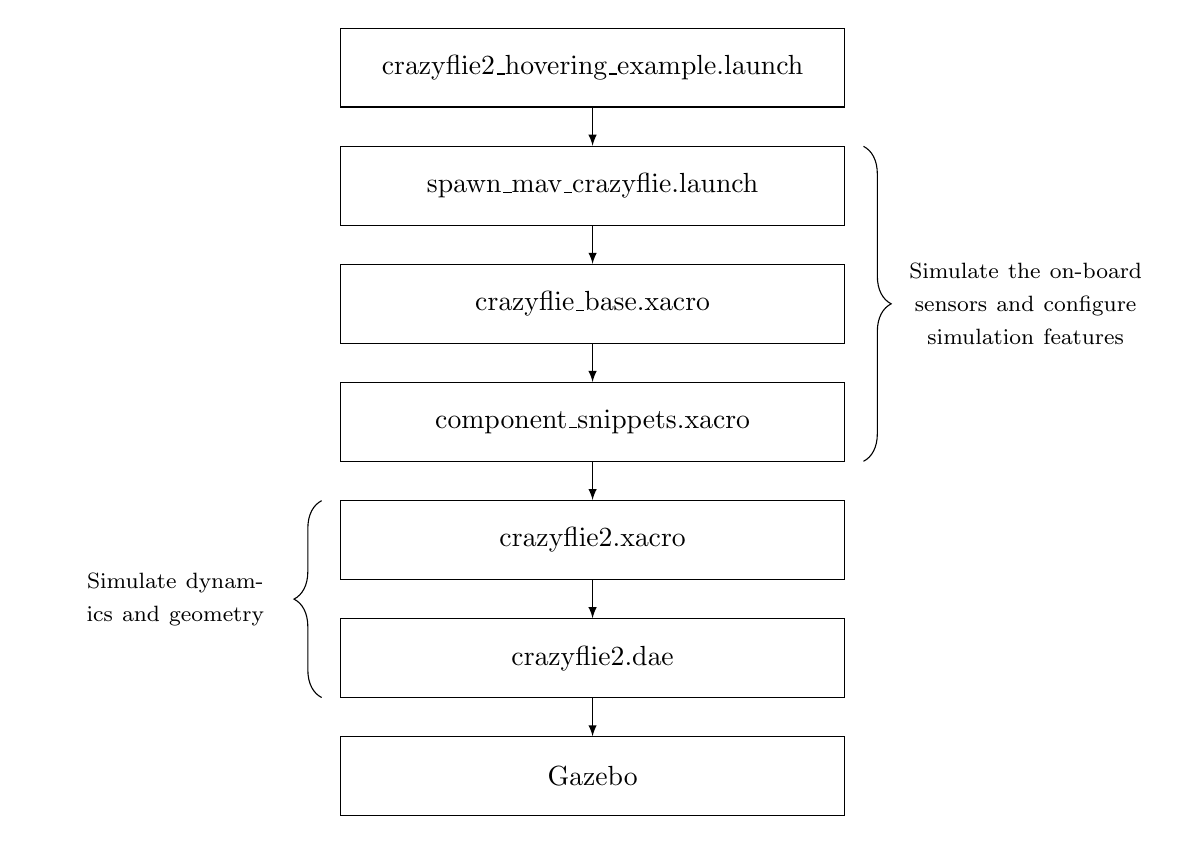
\begin{tikzpicture}
			
			%Rectangles
			\node (launchFile) at (0,0) [rectangle, draw, minimum width=6.4cm, minimum 
			height=1cm]{crazyflie2\_hovering\_example.launch};
			\node (spawnMav) at (0,-1.5) [rectangle, draw, minimum width=6.4cm, minimum 
			height=1cm]{spawn\_mav\_crazyflie.launch};
			\node (crazyflieBase) at (0,-3) [rectangle, draw, minimum width=6.4cm, minimum 
			height=1cm]{crazyflie\_base.xacro};
			\node (componentSnippets) at (0,-4.5) [rectangle, draw, minimum width=6.4cm, minimum 
			height=1cm]{component\_snippets.xacro};
			\node (crazyflieXacro) at (0,-6) [rectangle, draw, minimum width=6.4cm, minimum 
			height=1cm]{crazyflie2.xacro};
			\node (crazyflieDae) at (0,-7.5) [rectangle, draw, minimum width=6.4cm, minimum 
			height=1cm]{crazyflie2.dae};
			\node (gazebo) at (0,-9) [rectangle, draw, minimum width=6.4cm, minimum 
			height=1cm]{Gazebo};
			
			%Links among blocks
			\draw[-latex] (launchFile) -- (spawnMav);
			\draw[-latex] (spawnMav) -- (crazyflieBase);
			\draw[-latex] (crazyflieBase) -- (componentSnippets);
			\draw[-latex] (componentSnippets) -- (crazyflieXacro);
			\draw[-latex] (crazyflieXacro) -- (crazyflieDae);
			\draw[-latex] (crazyflieDae) -- (gazebo);
			
			%Curly brackets
			\draw [decorate,decoration={brace,amplitude=10pt,raise=4pt},yshift=0pt]
			(3.3,-1) -- (3.3,-5) node [black,midway,xshift=2.2cm, text centered, text width=10em] 
			{\footnotesize
				Simulate the on-board sensors and configure simulation features};
			\draw [decorate,decoration={brace,amplitude=10pt, mirror, raise=4pt},yshift=0pt]
			(-3.3,-5.5) -- (-3.3,-8) node [black,midway,xshift=-2cm, text width=10em, text 
			centered] {\footnotesize
				Simulate dynamics and geometry};
			\end{tikzpicture}
		}
	\end{center}
\end{figure}

%%%%%%%%%%%%%%%%%%%%%%%%%%%%%%%%%%%%%%%%%%%%%%%%%%%%%%%%%%%%%%%%%%%%%%%%%%%%%%%%%%%%%%%%%%%%%%%%%%%%

\section{Example \theblockDiagram}
\stepcounter{blockDiagram}

\begin{figure}[h]
	\begin{center}
		\scalebox{1}{
			\begin{tikzpicture}
			
			%Scheme blocks
			\node (outerLoop) at (-0.25,0) [draw, rectangle, minimum width=1cm,	minimum 
			height=1.5cm, text centered, text width=5em]{Outer loop\\controller};
			\node (innerController) at (2.6,-0.75) [draw, rectangle, minimum width=1cm, 
			minimum height=1.5cm, text centered, text width=5em]{Inner loop\\controller};
			\node (controlMixer) at (5.9,0) [draw, rectangle, minimum width=1cm, minimum 
			height=1.5cm, text centered, text width=5em]{Control\\Mixer};
			\node (bebopModel) at (10,0) [draw, rectangle, minimum width=1cm, minimum 
			height=1.5cm, text centered, text width=5em]{Aircraft\\+ \\ Motors};
			
			%Links between blocks
			\draw[-latex] ($ (outerLoop.160) - (1,0) $) -- node[above]{$\xi_r$} (outerLoop.160);
			\draw[-latex] ($ (outerLoop.200) - (1,0) $) -- node[above]{$\psi_r$} (outerLoop.200);
			\draw[fill=black] (-1.88,-0.4) arc(-180:180:0.03);
			
			\draw[-] (-1.85,-0.425) -- (-1.85, -1.155) -- (-0.35, -1.155);
			\draw[-] (-0.35,-1.155) arc (180:0:0.1);
			\draw[-latex]($ (innerController.200) - (1.65,0) $) -- node[below]{$\psi_r$} 
			(innerController.200);
			
			\draw[-latex] ($ (outerLoop.south) - (0,0.75) $) node[left]{$\xi_d$} -- 
			(outerLoop.south);
			\draw[-latex] (outerLoop.20) node[above right]{$u_T$} -- (controlMixer.160);
			\draw[-latex] ($ (innerController.160) - (0.67,0) $) node[above right]{$\varphi_r$} 
			node[below right]{$\theta_r$} -- (innerController.160); 
			\draw[-latex] ($ (controlMixer.201) - (1.11,0) $) -- node[above]{$u_\varphi$, 
			$u_\theta$} node[below]{$u_\psi$} (controlMixer.201);
			\draw[-latex] ($ (innerController.south) - (0,0.45) $) node[left]{$\eta_d$} -- 
			(innerController.south);
			\draw[-] ($ (innerController.south) - (0,0.45) $) -- ++(9.25,0) --  ++(0,1.58);
			\draw[fill=black] (11.83,-0.39) arc(-180:180:0.02);
			
			
			\draw[-] ($ (outerLoop.south) - (0,0.5) $) -- ++(0,-0.87) -- ++	(11.5,0) --  
			++(0,1.675);
			\draw[-] (11.245,-0.45) arc(-90:90:0.1) -- ++(0,0.64);
			\draw[fill=black] (11.23,0.40) arc(-180:180:0.02);
			
			\draw[-latex] (controlMixer) -- node[above]{$\Omega_{1}^\mathrm{ref}$, 
			$\Omega_{2}^\mathrm{ref}$} node[below]{$\Omega_{3}^\mathrm{ref}$, 
			$\Omega_{4}^\mathrm{ref}$} (bebopModel);
			\draw[-latex] (bebopModel.20) -- node[above]{$\xi_d$} ($(bebopModel.20) + 
			(1.2,0)$);
			\draw[-latex] (bebopModel.-20) --  node[above]{$\eta_d$} ($(bebopModel.-20) + 
			(1.2,0) $);
			
			\end{tikzpicture}
		}
	\end{center}
\end{figure}

\newpage

%%%%%%%%%%%%%%%%%%%%%%%%%%%%%%%%%%%%%%%%%%%%%%%%%%%%%%%%%%%%%%%%%%%%%%%%%%%%%%%%%%%%%%%%%%%%%%%%%%%%

\section{Example \theblockDiagram}
\stepcounter{blockDiagram}

\begin{figure}[h]
	\begin{center}
		\begin{tikzpicture}[>=stealth',shorten >=1pt,node distance=2cm,on grid,auto] 
		
		%Automata states
		\node[state] (q_1)   {$x_1$}; 
		\node[state] (q_2) [below left=of q_1] {$x_2$}; 
		\node[state] (q_3) [below right=of q_1] {$x_3$};
		\node[state] (q_4) [below=of q_2] {$x_4$};
		
		%Paths
		\path[->] 
		(q_1) edge              node        {$\sigma_1$}  (q_3)
		edge              node [swap] {$\sigma_1$}  (q_2)
		(q_2) edge [bend left]  node [swap] {$\sigma_2$}  (q_3)
		edge [loop left]  node        {$\sigma_1$}  ()
		edge [bend right] node [swap] {$\sigma_2$}  (q_4)
		(q_3) edge [bend left]  node        {$\sigma_1$}  (q_2)
		edge [loop right] node        {$\sigma_2$}  ()
		(q_4) edge [bend right] node        {$\sigma_1$}  (q_2)
		edge [loop right] node        {$\sigma_1$}  ();
		
		%Automata states
		\node[state] (q_5)  at (6,0)  {$x_1$}; 
		\node[state] (q_6) [below left=of q_5] {$x_2$}; 
		\node[state] (q_7) [below right=of q_5] {$x_3$};
		
		%Paths
		\path[->] 
		(q_5) edge              node        {$\sigma_1$}  (q_7)
		edge              node [swap] {$\sigma_1$}  (q_6)
		(q_6) edge [bend left]  node [swap] {$\sigma_2$}  (q_7)
		edge [loop left]  node        {$\sigma_1$}  ()
		edge [loop below] node        {$\sigma_2$}  ()
		(q_7) edge [bend left]  node        {$\sigma_1$}  (q_6)
		edge [loop right] node        {$\sigma_2$}  ();
		
		\end{tikzpicture}
	\end{center}
\end{figure}

%%%%%%%%%%%%%%%%%%%%%%%%%%%%%%%%%%%%%%%%%%%%%%%%%%%%%%%%%%%%%%%%%%%%%%%%%%%%%%%%%%%%%%%%%%%%%%%%%%%%

\section{Example \theblockDiagram}
\stepcounter{blockDiagram}

\begin{figure}[h]
	\begin{center}
		\scalebox{1}{
			\begin{tikzpicture}
			[>=stealth',shorten >=1pt,node distance=2cm,on grid,auto] 
			
			%Automata states
			\node[state] (q_0) {$p,\,r$}; 
			\node[state] (q_1) [above right= of q_0] {$r$}; 
			\node[state] (q_2) [above left= of q_0] {$p,\,q$};
			\node[state] (q_3) [below of= q_1] {$p$};
			\node[state] (q_4) [below left= of q_0] {$p$};
			\node[state] (q_5) [below left of= q_3] {$p,\,q$};
			
			\path[->] 
			(q_0) edge [bend right] node        {} (q_1)
			edge [bend right] node [swap] {} (q_2)
			edge [bend right] node        {} (q_4)
			(q_1) edge [bend left]  node [swap] {} (q_3)
			(q_2) edge [bend right]  node [swap] {} (q_0)
			(q_3) edge [bend left]  node        {} (q_5)
			edge [bend left]  node [swap] {} (q_0)
			(q_5) edge [bend left]  node [swap] {} (q_0)
			(q_4) edge [bend right] node [swap] {} (q_5);
			
			\end{tikzpicture}
		}
	\end{center}
\end{figure}

\newpage

%%%%%%%%%%%%%%%%%%%%%%%%%%%%%%%%%%%%%%%%%%%%%%%%%%%%%%%%%%%%%%%%%%%%%%%%%%%%%%%%%%%%%%%%%%%%%%%%%%%%

\section{Example \theblockDiagram}
\stepcounter{blockDiagram}

\begin{figure}[h]
	\begin{center}
		\begin{tikzpicture}
		
		% Nodes
		\node (MIL) at (0,0) [draw, rectangle, text centered, minimum width=1cm]{MIL};
		\node (SIL) at (0,-2) [draw, rectangle, text centered, minimum width=1cm]{SIL};
		\node (HIL) at (0,-4) [draw, rectangle, text centered, minimum width=1cm]{HIL};
		
		\node (testModel) at (-3,0) [draw, rectangle, text centered, minimum width=1cm]{Test Model};
		\node (code) at (-3,-2) [draw, rectangle, text centered, minimum width=1cm]{Code};
		
		\node (testSignal) at (-6,-1) [draw, rectangle, text centered, minimum width=1cm]{Test 
			Signal};
		
		\node (compareResults) at (3,-2) [draw, rectangle, text centered, minimum width=1cm, text 
		width=5em]{Compare\\results};
		
		% Links
		\draw[-latex] (code) -- (SIL);
		\draw[-latex] (testModel) -- (MIL);
		\draw[-latex, dashed] (testModel.south) -- node[right, text width=5em, text centered] 
		{Code\\generation} (code.north);
		\draw[-latex] (testSignal) -| ($ (testModel) - (1.5,0)$) -- (testModel);
		\draw[-latex] (testSignal) -| ($ (code) - (1.5,0)$) -- (code);
		\draw[-latex] (code) |- (HIL);
		
		\draw[-latex] (HIL) node at ($ (HIL) + (1,0.5)$) [text centered] 
		{\includegraphics[scale=0.05]{figure/hardware}} -| 
		(compareResults);
		\draw[-latex] (SIL) node at ($ (SIL) + (1,0.5)$) [text centered] 
		{\includegraphics[scale=0.075]{figure/PC}}-- (compareResults);
		\draw[-latex] (MIL) node at ($ (MIL) + (1,0.5)$) [text centered] 
		{\includegraphics[scale=0.075]{figure/PC}} -| (compareResults);
		
		\draw[-latex] (compareResults) -- ( $(compareResults) + (2,0)$ );
		
		\end{tikzpicture}
	\end{center}
\end{figure}	

%%%%%%%%%%%%%%%%%%%%%%%%%%%%%%%%%%%%%%%%%%%%%%%%%%%%%%%%%%%%%%%%%%%%%%%%%%%%%%%%%%%%%%%%%%%%%%%%%%%%

\section{Example \theblockDiagram}
\stepcounter{blockDiagram}	

\begin{figure}[h]
	\begin{center}
		\scalebox{0.825}{
			\begin{tikzpicture}
			
			% Feedback Linearization block
			\node (feedbackLinearization) at (0,0) [draw, minimum height=2cm, minimum 
			width=1cm, text width=4em, text centered]{Feedback\\Lineariz.};
			
			% Virtual inputs
			\node (virtualInputs) at (-3,1.25) [draw, minimum height=2cm, minimum 
			width=1cm, text width=4em, text centered]{Virtual\\Inputs};
			
			% Outputs and derivatives
			\node (outputDerivatives) at (-5.5,-2) [draw, minimum height=2cm, minimum 
			width=1cm, text width=4em, text centered]{Outputs\\\&\\Derivativ.};
			
			% Dynamical model
			\node (dynamicalSystem) at (4.85,0) [draw, minimum height=2cm, minimum 
			width=1cm, text width=4em, text centered]{Dynamic \\System};
			
			% Add blocks
			\node (sum1) at ($ (outputDerivatives.60) + (0,2) $) [draw, circle, text centered, 
			minimum size=0.5cm]{};
			\draw ($ (sum1) + (0.15,0.15) $) coordinate node[above left]{$+$};
			\draw ($ (sum1) + (-0.05,-0.1) $) coordinate node[below right]{$-$};
			\node (sum2) at ($ (outputDerivatives.120) + (0,2.75) $) [draw, circle, text centered, 
			minimum size=0.5cm]{};
			\draw ($ (sum2) + (0.15,0.15) $) coordinate node[above left]{$+$};
			\draw ($ (sum2) + (-0.05,-0.1) $) coordinate node[below right]{$-$};
			
			% Integrators
			\node (integrator1) at (1.86,-0.25) [draw, text centered]{$\int$};
			\node (integrator2) at (3,-0.25) [draw, text centered]{$\int$};
			
			%%%%%%% Links
			% Virtual Inputs
			\draw[-latex]{} (virtualInputs.-40) -- node[above, text centered, yshift=-0.1cm] 
			{$\mathbf{v}_2$} ($ (virtualInputs.-40) + (1.05,0) $);
			\draw[-latex]{} (virtualInputs.-25) -- node[above, text centered, yshift=-0.1cm] 
			{$\mathbf{v}_1$} ($	(virtualInputs.-25) + (1.05,0) $);
			\draw[-latex] ($ (virtualInputs.70) + (0,1) $) -- 
			node[right]{$\bm{\varphi}^{d(4)}$} (virtualInputs.70);
			\draw[-latex] ($ (virtualInputs.110) + (0,1) $) -- 
			node[left]{${^B\mathbf{\ddot{f}}}_L^d$} 
			(virtualInputs.110);
			\draw[-latex] (sum1) -- node[above]{$\mathbf{e}_{f_L}$} ($ (sum1) + (0.95,0)$);
			\draw[-latex] (sum2) -- node[above]{$\mathbf{e}_{\varphi}$} ($ (sum2) + (2.08,0)$);
			\draw[-latex] ($ (sum2) - (1,0)$) -- (sum2);
			\draw ($ (sum2) - (1.35,0)$) coordinate node [above]{$\bm{\varphi}^d$, \dots, 
				$\bm{\dddot{\varphi}}^d$};
			\draw[-latex] ($ (sum1) - (1,0)$) -- (sum1);
			\draw ($ (sum1) - (0,0)$) node[below, text width=5em]{$\Scale[1]{{^B\mathbf{f}}^d_L}$,\\
				$\Scale[1]{{^B\mathbf{\dot{f}}}^d_L}$};
			
			% Integrators
			\draw[-latex] ($ (integrator1) - (0.89,0) $) -- (integrator1);
			\draw ($ (integrator1) - (0.6,0) $) 
			node[above]{$\Scale[0.8]{{^B\mathbf{\ddot{f}}}_R}$};
			\draw[-latex] (integrator1) -- node[above]{$\Scale[0.8]{{^B\mathbf{\dot{f}}}_R}$} 
			(integrator2);
			\draw[-latex] (integrator2) -- node[above]{$\Scale[0.8]{{^B\mathbf{f}}_R}$} ($ 
			(integrator2) + (0.88,0) $);
			
			% From integrators to Outputs and Derivatives
			\draw[-latex] ($ (integrator1) - (0.65,0) $) |- (outputDerivatives.-25);
			\draw[fill=black] ($ (integrator1) - (0.69,0) $) arc(-180:180:0.04);
			\draw[-latex] ($ (integrator2) + (0.45,0) $) |- (outputDerivatives.-40);
			\draw[fill=black] ($ (integrator2) + (0.41,0) $) arc(-180:180:0.04);
			
			% Dynamic System
			\draw[-latex] (feedbackLinearization.30) -- node[above, text centered, yshift=-0.1cm] 
			{$^B\bm{\tau}_R$} (dynamicalSystem.150);
			
			% From Outputs & Derivatives to Add blocks
			\draw[-latex] (outputDerivatives.60) node at ($ (outputDerivatives.60) + (0,0.75) $) 
			[right]{${^B\mathbf{f}}_L$, ${^B\mathbf{\dot{f}}}_L$} 
			-- (sum1);
			\draw[-latex] (outputDerivatives.120) node at ($ (outputDerivatives.120) + (0,0.75) 
			$)[left]{$\bm{\varphi}$, \dots, $\bm{\dddot{\varphi}}$} -- (sum2);
			\draw[-latex] ($ (outputDerivatives.0) + (1,0) $) -- node[above]{$\mathbf{x}$} 
			(outputDerivatives.0);
			
			% To Feedback Linearization block
			\draw[-latex] ($ (feedbackLinearization.290) + (0,-1.46) $) --  
			(feedbackLinearization.290);
			\draw[fill=black] ($ (feedbackLinearization.290) + (-0.04,-1.46) $) arc(-180:180:0.04);
			\draw[-latex] ($ (feedbackLinearization.250) + (0,-1.82) $) --  
			(feedbackLinearization.250);
			\draw[fill=black] ($ (feedbackLinearization.250) + (-0.04,-1.82) $) arc(-180:180:0.04);
			\draw[-latex] ($ (feedbackLinearization.200) + (-1,0) $) -- node[above]{$\mathbf{x}$} 
			(feedbackLinearization.200);
			
			
			\end{tikzpicture}
		}
	\end{center}
\end{figure}

\newpage

%%%%%%%%%%%%%%%%%%%%%%%%%%%%%%%%%%%%%%%%%%%%%%%%%%%%%%%%%%%%%%%%%%%%%%%%%%%%%%%%%%%%%%%%%%%%%%%%%%%%

\section{Example \theblockDiagram}
\stepcounter{blockDiagram}	

\begin{figure}[h]
	\begin{center}
		\scalebox{0.7}{
			\begin{tikzpicture}
			
			%%%% Blocks
			% Reference trajectory generator
			\node (referenceTrajectory) at (-5.6,0) [draw, rectangle, text centered, minimum 
			height=1.25cm, minimum width=1cm, text width=6em]{Trajectory\\Generator};
			
			% Controller algorithm
			\node (controller) at (0,-1.75) [draw, rectangle, text centered, minimum height=1.25cm, 
			minimum width=1cm, text width=6em]{Feed. Linea.\\Controller};
			
			% PID Controller
			\node (pidController) at (0,1.75) [draw, rectangle, text centered, minimum 
			height=1.25cm, minimum width=1cm, text width=6em]{PD \\Controller};
			
			% Dynamic system + rotor dynamics
			\node (dynamicSystem) at (5,0) [draw, rectangle, text centered, minimum 
			height=1.25cm, minimum width=1cm, text width=6em]{Syst. \& Rot.\\Dynamics};
			
			% State observer
			\node (stateObserver) at (0,-4.25) [draw, rectangle, text centered, minimum 
			height=1.25cm, minimum width=1cm, text width=6em]{State\\Observer};
			
			% Odometry sensor
			\node (odometrySensor) at (4.25,-4.25) [draw, rectangle, text centered, minimum 
			height=1.25cm, minimum width=1cm, text width=6em]{Odometry\\Sensor};
			
			% State observer2
			\node (stateObserver2) at (0,4.25) [draw, rectangle, text centered, minimum 
			height=1.25cm, minimum width=1cm, text width=6em]{State\\Observer};
			
			% Odometry sensor
			\node (odometrySensor2) at (4.25,4.25) [draw, rectangle, text centered, minimum 
			height=1.25cm, minimum width=1cm, text width=6em]{Odometry\\Sensor};
			
			\node (dashedBoxGazebo1) at (5,0) [draw, dashed, rectangle, text centered, 
			minimum height=1.75cm, minimum width=3.5cm]{};
			
			\node (dashedBoxGazebo) at (4.25,-4.25) [draw, dashed, rectangle, text centered, 
			minimum height=1.75cm, minimum width=3.25cm]{};
			
			\node (dashedBoxGazebo) at (4.25,4.25) [draw, dashed, rectangle, text centered, 
			minimum height=1.75cm, minimum width=3.25cm]{};
			
			% Gazebo text
			\draw (4.25,5.4) coordinate node [text centered]{Gazebo}; % Odometry sensor2
			\draw (4.25,-3.1) coordinate node [text centered]{Gazebo}; % Odometry sensor1
			\draw (5,1.15) coordinate node [text centered]{Gazebo};
			
			%%%% Links
			\draw[-latex] (referenceTrajectory) -- ($ (referenceTrajectory) + (3.85,0) $) |-  
			(controller);
			\draw[-latex] ($ (referenceTrajectory) + (3.85,0) $) |-  (pidController);
			\draw ($ (referenceTrajectory) + (2.65,0) $) coordinate node[above, text centered, text 
			width=5em]{$\bm{\varphi}^d$, $\dots$, \\ $\bm{\varphi}^{(4)d}$};
			\draw ($ (referenceTrajectory) + (2.65,0) $) coordinate 
			node[below, text width=5em, text centered]{${^B\mathbf{f}}_L^d$, 
				${^B\mathbf{f}}_L^{(1)d}$, \\ ${^B\mathbf{f}}_L^{(2)d}$};
			\draw[fill=black] ($ (referenceTrajectory) + (3.81,0) $) arc(-180:180:0.04);
			
			\draw[-] (controller) -- ($ (controller) + (2.35,0)$) -- node[left]{${^B\bm{\tau}}_R$} 
			node[right]{${^B\mathbf{f}}_R$} ($ (controller) + (2.35,1)$);
			\draw[-] (pidController) -- ($ (pidController) + (2.35,0)$) -- 
			node[left]{${^B\bm{\bar{\tau}}}_R$} node[right]{${^B\mathbf{\bar{f}}}_R$} ($ 
			(pidController) + (2.35,-1)$);
			\draw[latex-] ($(controller) + (2.35,1)$) to [bend left ]($(pidController) + 
			(2.35,-1)$);
			\draw[-latex] ($ (pidController) + (0.85,-1.75)$) -- node[above]{$\bar{A}$} 
			($ (pidController) + (2.1,-1.75)$);
			
			\draw[-latex] (stateObserver) -- node[left]{$\bm{\hat{\varphi}}$, 
				$\bm{\dot{\hat{\varphi}}}$} node[right]{$\bm{\hat{\vartheta}}$, 
				$\bm{\dot{\hat{\vartheta}}}$} (controller);
			
			\draw[-latex] (stateObserver2) -- node[left]{$\bm{\hat{\varphi}}$, 
				$\bm{\dot{\hat{\varphi}}}$} node[right]{$\bm{\hat{\vartheta}}$, 
				$\bm{\dot{\hat{\vartheta}}}$} (pidController);
			
			\draw[-latex] ($ (controller) + (0,1.5)$) -- node[left]{$\bar{A}$}(controller);
			\draw[-latex] ($ (pidController) - (0,1.5)$) -- node[left]{$A$}(pidController);
			
			\draw[-] ($ (pidController) + (2.35,-1)$) -- ($ (pidController) + (2.95,-1.75)$);
			\draw[-latex] ($ (pidController) + (2.95,-1.75)$) -- (dynamicSystem);
			\draw[fill=black] ($ (pidController) + (2.31,-1)$) arc(-180:180:0.04);
			\draw[fill=black] ($(controller) + (2.31,1)$) arc(-180:180:0.04);
			
			\draw[-latex] (odometrySensor) -- node[above]{${^W\mathbf{r}}_B$} 
			node[below]{$\bm{\vartheta}$} (stateObserver);
			\draw[-latex] (odometrySensor2) -- node[above]{${^W\mathbf{r}}_B$} 
			node[below]{$\bm{\vartheta}$} (stateObserver2);
			
			\end{tikzpicture}
		}
	\end{center}
\end{figure}

%%%%%%%%%%%%%%%%%%%%%%%%%%%%%%%%%%%%%%%%%%%%%%%%%%%%%%%%%%%%%%%%%%%%%%%%%%%%%%%%%%%%%%%%%%%%%%%%%%%%

\section{Example \theblockDiagram}
\stepcounter{blockDiagram}	

\begin{figure}[h]
	\begin{center}
	\scalebox{0.9}{
		\begin{tikzpicture}
		
		% Nodes
		\node (STLSpecifications) at (0,0) [text centered, draw, rectangle, minimum 
		width=4.5cm]{STL Specification};
		\node (ControlSTL) at (0,-1) [text centered, draw, rectangle, minimum 
		width=4.5cm]{High-level Control for STL};
		
		% Links
		\draw[-latex] (STLSpecifications) -- node[right]{$\varphi$} (ControlSTL);
		
		% Multi-robots box
		\node (MultiRobots-Box) at (0,-0.5) [draw, dashed, gray, minimum height=2cm, minimum 
		width=5.5cm]{}; 
		\draw[fill=black] ($ (ControlSTL.south) - (0.03,0.35) $) arc(-180:180:0.03);
		
		% Dots
		\node (Dots1) at (-1.35,-4.0) [text centered]{\dots};
		\node (Dots2) at (1.40,-4.0) [text centered]{\dots};
		
		%%%%%%%%%%%%%%%%%%%
		% Drone 1
		\node (TrajectoryGenerator1) at (-2.75,-2.6) [draw, rectangle, text centered, text 
		width=5em]{Trajectory\\Generator};
		\node (DroneController1) at (-2.75,-3.95) [draw, rectangle, text centered, text 
		width=5em]{Drone\\Controller};
		\node (UAVDynamics1) at (-2.75,-5.35) [draw, rectangle, text centered, text 
		width=5em]{UAV\\Dynamics};
		\node (Drone-Box1) at (-2.75,-3.95) [draw, dashed, gray, minimum height=4.1cm, minimum 
		width=2.35cm]{}; 
		\node (Drone-Box1-Text) at (-2.75,-6.35) [text centered]{$1$-quadrotor};	
		
		% Drone 1 - Links
		\draw[-latex] (TrajectoryGenerator1) -- node[left]{$\pmb{\xi}_1$} 
		node[right]{$\pmb{\eta}_1$} (DroneController1);
		\draw[-latex] (DroneController1) -- node[left]{$\pmb{\Omega}_1$} (UAVDynamics1);	
		\draw[-latex] (ControlSTL.south) -- ($ (ControlSTL.south) - (0,0.35) $) -- ($ 
		(ControlSTL.south) - (2.75,0.35) $) -- node[above left]{$^W\mathbf{r}_1$, $\psi_1$} 
		(TrajectoryGenerator1.north);
		
		%%%%%%%%%%%%%%%%%%%
		% Drone 2
		\node (TrajectoryGenerator2) at (0,-2.6) [draw, rectangle, text centered, text 
		width=5em]{Trajectory\\Generator};
		\node (DroneController2) at (0,-3.95) [draw, rectangle, text centered, text 
		width=5em]{Drone\\Controller};
		\node (UAVDynamics2) at (0,-5.35) [draw, rectangle, text centered, text 
		width=5em]{UAV\\Dynamics};
		\node (Drone-Box2) at (0,-3.95) [draw, dashed, gray, minimum height=4.1cm, minimum 
		width=2.35cm]{};
		\node (Drone-Box2-Text) at (0,-6.35) [text centered]{$2$-quadrotor};		
		
		% Drone 2 - Links
		\draw[-latex] (TrajectoryGenerator2) -- node[left]{$\pmb{\xi}_2$} 
		node[right]{$\pmb{\eta}_2$} (DroneController2);
		\draw[-latex] (DroneController2) -- node[left]{$\pmb{\Omega}_2$}(UAVDynamics2);	 
		\draw[-latex] ($ (ControlSTL.south) - (0,0.35) $) -- node[left]{$^W\mathbf{r}_2$, $\psi_2$} 
		(TrajectoryGenerator2.north);
		
		%%%%%%%%%%%%%%%%%%%
		% Drone N
		\node (TrajectoryGeneratorN) at (2.75,-2.6) [draw, rectangle, text centered, text 
		width=5em]{Trajectory\\Generator};
		\node (DroneControllerN) at (2.75,-3.95) [draw, rectangle, text centered, text 
		width=5em]{Drone\\Controller};
		\node (UAVDynamicsN) at (2.75,-5.35) [draw, rectangle, text centered, text 
		width=5em]{UAV\\Dynamics};	
		\node (Drone-BoxN) at (2.75,-3.95) [draw, dashed, gray, minimum height=4.1cm, minimum 
		width=2.35cm]{}; 	
		\node (Drone-BoxN-Text) at (2.75,-6.35) [text centered]{$n$-quadrotor};
		
		% Drone N - Links
		\draw[-latex] (TrajectoryGeneratorN) -- node[left]{$\pmb{\xi}_n$} 
		node[right]{$\pmb{\eta}_n$} (DroneControllerN);
		\draw[-latex] (DroneControllerN) -- node[left]{$\pmb{\Omega}_n$} (UAVDynamicsN);	
		\draw[-latex] ($ (ControlSTL.south) - (0,0.35) $) -- ($ (ControlSTL.south) + (2.75,-0.35) 
		$) -- node[above right]{$^W\mathbf{r}_n$, $\psi_n$} (TrajectoryGeneratorN.north);
		
		\end{tikzpicture}
		}
	\end{center}
\end{figure}